\documentclass[a5paper, 10pt]{article}

% Текст
\usepackage[utf8]{inputenc} % UTF-8 кодировка
\usepackage[russian]{babel} % Русский язык
\usepackage{indentfirst} % красная строка в первом параграфе в главе
% Отображение страниц
\usepackage{geometry} % размеры листа и отступов
\usepackage{listings}
\usepackage{color}
\setcounter{totalnumber}{10}
\setcounter{topnumber}{10}

\geometry{
	left=12mm,
	top=25mm,
	right=15mm,
	bottom=17mm,
	marginparsep=0mm,
	marginparwidth=0mm,
	headheight=10mm,
	headsep=7mm,
	nofoot}
\usepackage{afterpage,fancyhdr} % настройка колонтитулов
\pagestyle{fancy}
\fancypagestyle{style}{ % создание нового стиля style
	\fancyhf{} % очистка колонтитулов
	\fancyhead[LO, RE]{Лабораторная работа № 1 } % название документа наверху
	\fancyhead[RO, LE]{Ряды Фурье} % название section наверху
	\fancyfoot[RO, LE]{\thepage} % номер страницы справа внизу на нечетных и слева внизу на четных
	\renewcommand{\headrulewidth}{0.25pt} % толщина линии сверху
	\renewcommand{\footrulewidth}{0pt} % толцина линии снизу
}
\fancypagestyle{plain}{ % создание нового стиля plain -- полностью пустого
	\fancyhf{}
	\renewcommand{\headrulewidth}{0pt}
}
\fancypagestyle{title}{ % создание нового стиля title -- для титульной страницы
	\fancyhf{}
	\fancyhead[C]{{\footnotesize
			Министерство образования и науки Российской Федерации\\
			Федеральное государственное автономное образовательное учреждение высшего образования
	}}
	\fancyfoot[C]{{\large 
			Санкт-Петербург, 2024
	}}
	\renewcommand{\headrulewidth}{0pt}
}

% Математика
\usepackage{amsmath, amsfonts, amssymb, amsthm} % Набор пакетов для математических текстов
%\usepackage{dmvnbase} % мехматовский пакет latex-сокращений
\usepackage{cancel} % зачеркивание для сокращений
% Рисунки и фигуры
\usepackage[pdftex]{graphicx} % вставка рисунков
\usepackage{wrapfig, subcaption} % вставка фигур, обтекая текст
\usepackage{caption} % для настройки подписей
\captionsetup{figurewithin=none,labelsep=period, font={small,it}} % настройка подписей к рисункам
% Рисование
\usepackage{tikz} % рисование
\usepackage{circuitikz}
\usepackage{pgfplots} % графики
% Таблицы
\usepackage{multirow} % объединение строк
\usepackage{multicol} % объединение столбцов
% Остальное
\usepackage[unicode, pdftex]{hyperref} % гиперссылки
\usepackage{enumitem} % нормальное оформление списков
\setlist{itemsep=0.15cm,topsep=0.15cm,parsep=1pt} % настройки списков
% Теоремы, леммы, определения...
\theoremstyle{definition}
\newtheorem{Def}{Определение}
\newtheorem*{Axiom}{Аксиома}
\theoremstyle{plain}
\newtheorem{Th}{Теорема}
\newtheorem{Lem}{Лемма}
\newtheorem{Cor}{Следствие}
\newtheorem{Ex}{Пример}
\theoremstyle{remark}
\newtheorem*{Note}{Замечание}
\newtheorem*{Solution}{Решение}
\newtheorem*{Proof}{Доказательство}
% Свои команды
\newcommand{\comb}[1]{\left[\hspace{-4pt}\begin{array}{l}#1\end{array}\right.\hspace{-5pt} } % совокупность уравнений
% Титульный лист
\usepackage{csvsimple-l3}
\newcommand*{\titlePage}{
	\thispagestyle{title}
	\begingroup
	\begin{center}
		%		{\footnotesize
			%			Министерство образования и науки Российской Федерации\\
			%			Федеральное государственное автономное образовательное учреждение высшего образования
			%		}
		%		
		\vspace*{6ex}
		
		{\small
			САНКТ-ПЕТЕРБУРГСКИЙ НАЦИОНАЛЬНЫЙ ИССЛЕДОВАТЕЛЬСКИЙ УНИВЕРСИТЕТ ИТМО	
		}
		
		\vspace*{2ex}
		
		{\normalsize
			Факультет систем управления и робототехники
		}
		
		\vspace*{15ex}
		
		{\Large \bfseries 
			Лабораторная работа № 1
		}
\vspace*{2ex}
	{\Large \bfseries 
			
"Ряды Фурье"
		}
\vspace*{2ex}
		
		{\normalsize
			по дисциплине Частотные методы
		}

	\end{center}
	\vspace*{20ex}
	\begin{flushright}
		{\large 
			\underline{Выполнила}: студентка гр. \textbf{R3238}\\
			\begin{flushright}
				\textbf{Нечаева А. А.}\\
			\end{flushright}
		}
		
		\vspace*{5ex}
		
		{\large 
			\underline{Преподаватель}: \textit{Перегудин Алексей Алексеевич}
		}
	\end{flushright}	
	\newpage
	\setcounter{page}{1}
	\endgroup}

\begin{document}
	\titlePage
	\pagestyle{style}

\lstset{ %
language=C,                 % выбор языка для подсветки (здесь это С)
basicstyle=\small\sffamily, % размер и начертание шрифта для подсветки кода
numbers=left,               % где поставить нумерацию строк (слева\справа)
numberstyle=\tiny,           % размер шрифта для номеров строк
stepnumber=1,                   % размер шага между двумя номерами строк
numbersep=5pt,                % как далеко отстоят номера строк от подсвечиваемого кода
backgroundcolor=\color{white}, % цвет фона подсветки - используем \usepackage{color}
showspaces=false,            % показывать или нет пробелы специальными отступами
showstringspaces=false,      % показывать или нет пробелы в строках
showtabs=false,             % показывать или нет табуляцию в строках
frame=single,              % рисовать рамку вокруг кода
tabsize=2,                 % размер табуляции по умолчанию равен 2 пробелам
captionpos=t,              % позиция заголовка вверху [t] или внизу [b] 
breaklines=true,           % автоматически переносить строки (да\нет)
breakatwhitespace=false, % переносить строки только если есть пробел
escapeinside={\%*}{*)}   % если нужно добавить комментарии в коде
}



\newpage
\section{Задание. Вещественные функции.}
Придумать числа $a, \, b, \, t_0, \, t_1, \, t_2$ такие, что $a, \, b > 0$ и $t_2 > t_1 > t_0 > 0$. \\
Пусть $a = 1, \, b = 2; \, t_0 = \pi, \, t_1 = 2 \pi, \, t_2 = 3 \pi$. \\ Рассмотрим следующие функции $f\, : \mathbb{R} \to \mathbb{R}$:

\subsection{Квадратная волна.}
Периодическая функция с периодом $T=t_2 - t_0 = 3 \pi - \pi = 2 \pi$ такая, что 
\begin{equation}
f(t) =
\begin{cases}
a, \, \, t \in \, [t_0, \, t_1 ),\\
b, \, \, t \in \, [t_1, \, t_2 )
\end{cases}
= \,\,\,\,
\begin{cases}
1, \, \, t \in \, [\pi, \, 2 \pi ),\\
2, \, \, t \in \, [2 \pi, \, 3 \pi)
\end{cases}
\end{equation}

\subsubsection{График функции}
\begin{figure}[h]
\center{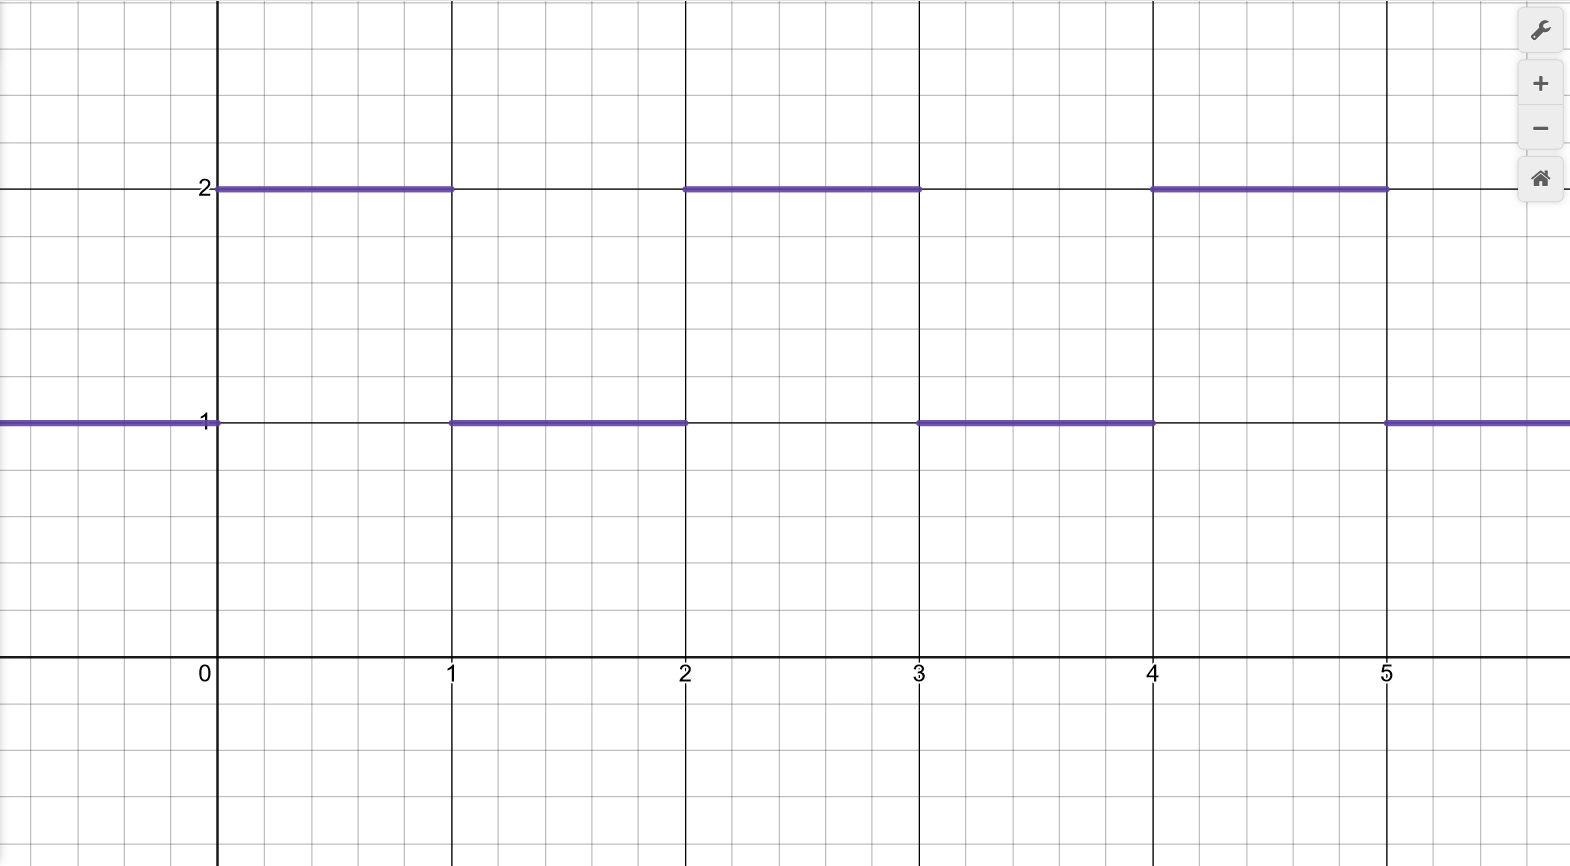
\includegraphics[width=0.9\linewidth]{pic/gr_1.png}}
\caption{График функции $f(t)$.}
\end{figure}

\subsubsection{Частичные суммы Фурье}
Рассмотрим частичные суммы Фурье $F_N$ и $G_N$ вида

\begin{equation}
F_N(t) = \frac{a_0}{2} + \sum  \limits_{n=1}^N \left( a_n \cos \left( \omega_n t \right) + b_n \sin \left( \omega_n t \right)  \right) \, ,
\end{equation}

\begin{equation}
G_N (t) = \sum  \limits_{n=-N}^N c_n e^{i \omega_n t} \, ,
\end{equation}
где $\omega_n = 2 \pi \frac{n}{T}$.\\
\\
Перепишем формулы выше с учетом того, что $T = 2 \pi$, следовательно  $\omega_n = 2 \pi \frac{n}{ 2 \pi} = n$:
\begin{equation}
F_N(t) = \frac{a_0}{2} + \sum  \limits_{n=1}^N \left( a_n \cos \left( n t \right) + b_n \sin \left( n t \right)  \right) \, ,
\end{equation}

\begin{equation}
G_N (t) = \sum  \limits_{n=-N}^N c_n e^{i n t}.
\end{equation}

Перейдем к разложению по формуле 4.\\
$f(x)$ определена на $[ \pi, 3\pi]$, преобразуем:
\begin{equation}
\pi \leq t \leq 3 \pi \to \pi - 2 \pi \leq t - 2 \pi \leq 3 \pi - 2 \pi \to -\pi \leq t - 2 \pi \leq \pi
\end{equation}
Новая переменная $x = t - 2\pi$. Выразим $t = x + 2 \pi$ и запишем новую функцию $\phi (x) = f (x + 2 \pi)$.
\begin{equation}
\phi (x) = \frac{a_0}{2} + \sum  \limits_{n=1}^N \left( a_n \cos \left( n x \right) + b_n \sin \left( n x \right)  \right) \, ,
\end{equation}
где $a_0, \, a_n, \, b_n$ -- коэффициенты Фурье:

\subsubsection{Вычисление коэффициентов $a_n$, $b_n$ и $c_n$}
\begin{equation}
a_0 = \frac{1}{\pi} \int \limits_{-\pi}^{\pi} \phi (x) dx,
\end{equation}
\begin{equation}
a_n = \frac{1}{\pi} \int \limits_{-\pi}^{\pi} \phi (x) \cos (n x) dx,
\end{equation}
\begin{equation}
b_n = \frac{1}{\pi} \int \limits_{-\pi}^{\pi} \phi (x) \sin (nx) dx,
\end{equation}

Проведем обратную замену $x = t - 2\pi$:

\begin{equation}
f(t) = \frac{a_0}{2} + \sum  \limits_{n=1}^N \left( a_n \cos \left( n ( t - 2\pi) \right) + b_n \sin \left( n ( t - 2\pi) \right)  \right)
\end{equation}
Воспользуемся периодичностью синуса и косинуса:
\begin{equation}
f(t) = \frac{a_0}{2} + \sum  \limits_{n=1}^N \left( a_n \cos \left( n t  \right) + b_n \sin \left( n  t  \right)  \right)
\end{equation}
\begin{equation}
a_0 = \frac{1}{\pi} \int \limits_{\pi}^{3\pi} f(t) dt,
\end{equation}
\begin{equation}
a_n = \frac{1}{\pi} \int \limits_{\pi}^{3\pi} f(t) \cos (n t) dt,
\end{equation}
\begin{equation}
b_n = \frac{1}{\pi} \int \limits_{\pi}^{3\pi} f(t) \sin (nt) dt,
\end{equation}
Вычислим значения коэффициентов:

\begin{equation}
a_0 = \frac{1}{\pi} \left( \int \limits_{\pi}^{2\pi} 1 dt + \int \limits_{2\pi}^{3\pi} 2 dt\right) =
 \frac{1}{\pi} \left( \pi + 2\pi \right) = 3,
\end{equation}

\begin{equation}
a_n = \frac{1}{\pi} \left( \int \limits_{\pi}^{2\pi} \cos (n t) dt +  2\int \limits_{2\pi}^{3\pi} \cos (n t) dt \right)
\end{equation}

Отдельно вычислим неопределенный интеграл:
\begin{equation}
\int \cos (n t) dt = \left| u = nt , t = \frac{u}{n},  dt = \frac{du}{n}\right| = \int  \frac{ \cos (u) du}{n} = \frac{\sin u}{n} + C = \frac{\sin (nt)}{n} + C
\end{equation}


Отсюда получим
\begin{equation}
a_n = \frac{1}{\pi} \left( \left. \frac{\sin (nt)}{n} \right|_{\pi}^{2\pi} +  2  \left. \frac{\sin (nt)}{n} \right|_{2\pi}^{3\pi} \right) = 0
\end{equation}



\begin{multline}
b_n = \frac{1}{\pi} \left( \int \limits_{\pi}^{2\pi} \sin (n t) dt +  2\int \limits_{2\pi}^{3\pi} \sin (n t) dt \right) =
-\frac{1}{\pi} \left( \left. \frac{\cos (nt)}{n} \right|_{\pi}^{2\pi} +  2  \left. \frac{\cos (nt)}{n} \right|_{2\pi}^{3\pi} \right) =\\
= -\frac{1}{\pi} \left( \frac{\cos (2 \pi n) - \cos (\pi n)}{n} +  2 \frac{\cos (3 \pi n) - \cos (2 \pi n)}{n} \right) = \\
= -\frac{1}{\pi} \left( \frac{ 1 - \cos (\pi n)}{n} +  2 \frac{\cos (3 \pi n) - 1}{n} \right) =
-\frac{1}{\pi} \left( \frac{ 1 - (-1)^n}{n} +  2 \frac{(-1)^n - 1}{n} \right) =\\
= -\frac{1}{\pi} \left( \frac{(-1)^n - 1 }{n} \right) = \frac{1 - (-1)^n}{\pi n}
\end{multline}
Примеры вычисления первых значений $b_n$:
\begin{equation}
b_1 = \frac{1 - (-1)^1}{\pi} = \frac{2}{\pi}
\end{equation}
\begin{equation}
b_2 = \frac{1 - (-1)^2}{2\pi} = 0
\end{equation}
\begin{equation}
b_3 = \frac{1 - (-1)^3}{3\pi} = \frac{2}{3\pi}
\end{equation}
\begin{equation}
b_0 = \frac{1}{\pi} \left( \int \limits_{\pi}^{2\pi} \sin (0) dt +  2\int \limits_{2\pi}^{3\pi} \sin (0) dt \right)  = 0
\end{equation}

Запишем получившуюся частичную сумму:
\begin{equation}
F_N(t) = \frac{3}{2} + \sum  \limits_{n=1}^N \left( \frac{1 - (-1)^n}{\pi n} \sin \left( n t \right)  \right) \, ,
\end{equation}
\\
Перейдем к рассмотрению следующей частичной суммы:
\begin{equation}
G_N (t) = \sum  \limits_{n=-N}^N c_n e^{i n t}.
\end{equation}
Где соответствующий коэффициент:
\begin{equation}
c_n = \frac{1}{T} \int \limits_{h}^{h + T} f(t) e^{-i \omega_n t} dt = \frac{1}{2 \pi} \int \limits_{\pi}^{3 \pi} f(t) e^{-i n t} dt =
\frac{1}{2 \pi} \left( \int \limits_{\pi}^{2 \pi} e^{-i n t} dt + 2 \int \limits_{ 2 \pi}^{3 \pi} e^{-i n t} dt \right) 
\end{equation}

При $n=0$ коэффициент будет равен:
\begin{equation}
c_0 = \frac{1}{2 \pi} \left( \int \limits_{\pi}^{2 \pi} e^{0} dt + 2 \int \limits_{ 2 \pi}^{3 \pi} e^{0} dt \right) = \frac{3}{2}
\end{equation}

Отдельно вычислим неопределенный интеграл:
\begin{equation}
c_n = \int e^{-i n t} dt = \frac{-1}{in} \int e^{-i n t} d (-i n t) =  -\frac{e^{-i n t}}{in} + C
\end{equation}

\begin{equation}
c_n = -\frac{1}{2 \pi} \left(  \left. \frac{e^{-i n t}}{in} \right|_{\pi}^{2\pi} + 2  \left. \frac{e^{-i n t}}{in} \right|_{2\pi}^{3\pi} \right) =
 \frac{ e^{-i n \pi} + e^{-2i n \pi} - 2 e^{-3i n \pi}}{2 i n \pi}
\end{equation}


В итоге полученое разложение:
\begin{equation}
G_N (t) = \sum  \limits_{n=-N}^N   \frac{ e^{-i n \pi} + e^{-2i n \pi} - 2 e^{-3i n \pi}}{2 i n \pi} e^{i n t}.
\end{equation}


\subsubsection{Программа для вычисления коэффициентов Фурье}
Код для выисления коэффициентов Фурье написан на \textit{Python} с использованием библитеки $NumPy$.

\begin{center}
\begin{lstlisting}[label=some-code,caption={Функция, реализующая квадратную волну}]
def fun_square_wave(t):
    if (t // np.pi) % 2 == 0:
        return 2
    else:
        return 1


fun_wave = np.vectorize(fun_square_wave)
\end{lstlisting}
\end{center}

Необходимое в процессе нахождения коэффициентов интегрирование реализовано с помощью вычисления скалярного произведения подынтегральных функций.

\begin{center}
\begin{lstlisting}[label=some-code,caption={Функция, реализующая интегрирование для вычисления коэффициентов Фурье.}]
def integral_counter(f_1, f_2, a, b):

    t = np.linspace(a, b, my_sigma)
    dt = (b - a) / my_sigma

    return np.dot(f_1(t), f_2(t)) * dt
\end{lstlisting}
\end{center}

Далее приведены функции, непосредственно возвращающие вычисленные значения коэффициентов Фурье.

\begin{center}
\begin{lstlisting}[label=some-code,caption={Функция для коэффициентов $a_n$}]
def a_coef(f, N):
    res = []
    for n in range(N):
        fourier_cos = lambda t: np.cos(n * t)
        res.append(integral_counter(f, fourier_cos, np.pi, 3 * np.pi) / np.pi)

    return res
\end{lstlisting}
\end{center}


\begin{center}
\begin{lstlisting}[label=some-code,caption={Функция для коэффициентов $b_n$}]
def b_coef(f, N):
    res = []
    for n in range(N):
        fourier_sin = lambda t: np.sin(n * t)
        res.append(integral_counter(f, fourier_sin, np.pi, 3 * np.pi) / np.pi)
    return res
\end{lstlisting}
\end{center}


\begin{center}
\begin{lstlisting}[label=some-code,caption={Функция для коэффициентов $c_n$}]
def c_coef(f, N):
    res = []
    for n in range(N):
        fourier_exp = lambda t: np.exp(-1j * n * t)
        res.append(integral_counter(f, fourier_exp, np.pi, 3 * np.pi) / (2 * np.pi))
    return res
\end{lstlisting}
\end{center}

\begin{table}[h]
\caption{Значения коэффициентов, вычисленных с помощью написанной программы для квадратной волны.}
\label{tabular:timesandtenses}
\begin{center}
\begin{tabular}{|c|c|c|c|c|}
\hline
n & $a_n$ & $b_n$ & $Re(c_n)$ & $Im(c_n)$ \\
\hline
0 & 2.9998 & 0 & 1.4999 & 0\\
\hline
1 & -0.0001 & 0.6366 & -0.00005 & -0.3183\\
\hline
2 & 0.0001 & 0 & 0.00005  & 0\\
\hline
\end{tabular}
\end{center}
\end{table}

Значения коэффициентов для первых трех значений $n$, вычисленные с помощью программы близки к числам, полученным аналитически.

\subsubsection{Построение графиков частичных сумм $F_N$, $G_N$}

\begin{figure}[h]
\begin{minipage}[h]{0.5\linewidth}
\center{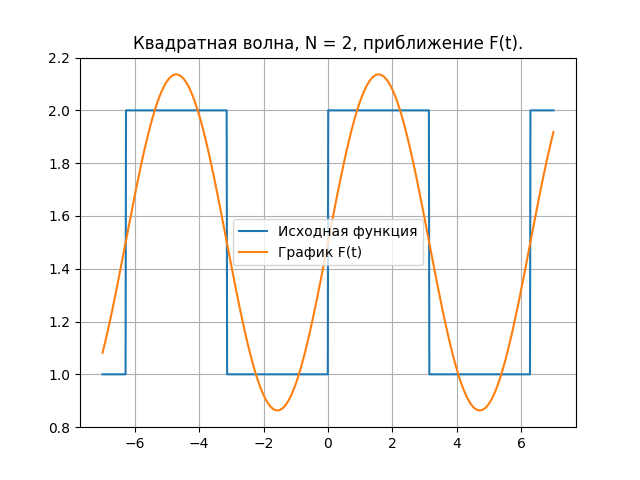
\includegraphics[width=1\linewidth]{gr_wave/f2.png} \\ а)}
\end{minipage}
\hfill
\begin{minipage}[h]{0.5\linewidth}
\center{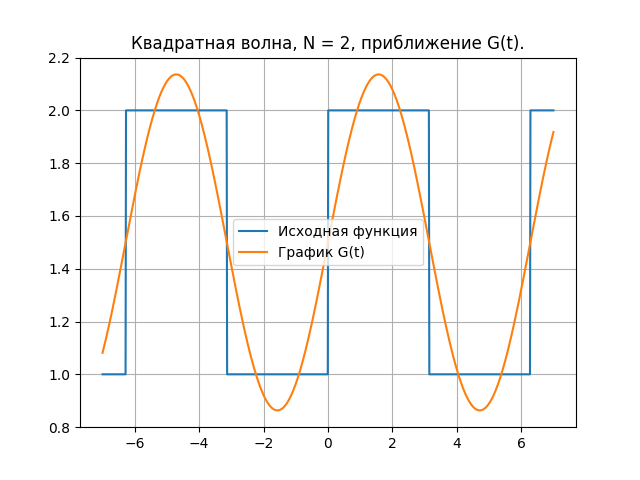
\includegraphics[width=1\linewidth]{gr_wave/g2.png} \\ б)}
\end{minipage}
\caption{Построение графиков частичных сумм, для квадратной волны, $N=2$.}
\end{figure}

\begin{figure}[h]
\begin{minipage}[h]{0.5\linewidth}
\center{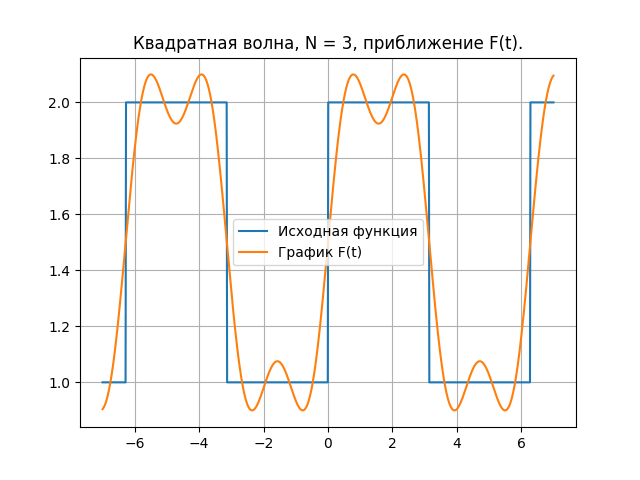
\includegraphics[width=1\linewidth]{gr_wave/f3.png} \\ а)}
\end{minipage}
\hfill
\begin{minipage}[h]{0.5\linewidth}
\center{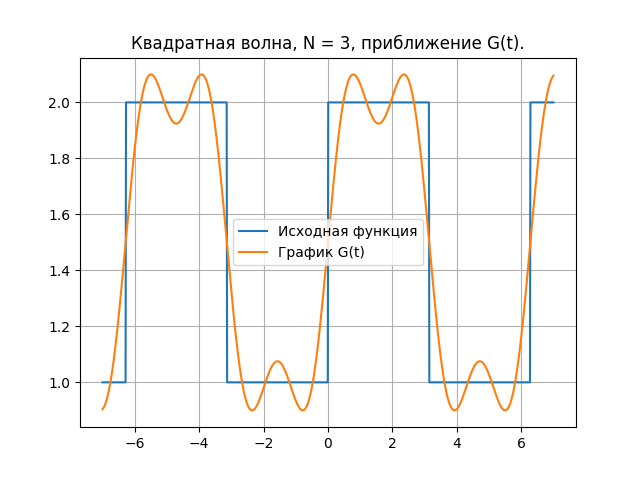
\includegraphics[width=1\linewidth]{gr_wave/g3.png} \\ б)}
\end{minipage}
\caption{Построение графиков частичных сумм, для квадратной волны, $N=3$.}
\vfill

\begin{minipage}[h]{0.5\linewidth}
\center{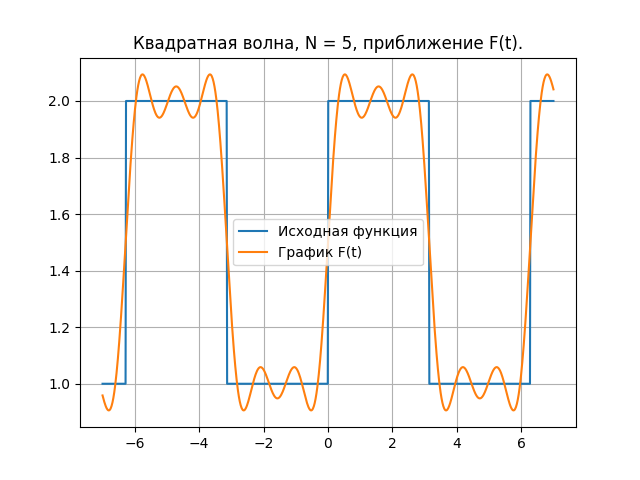
\includegraphics[width=1\linewidth]{gr_wave/f5.png} \\ а)}
\end{minipage}
\hfill
\begin{minipage}[h]{0.5\linewidth}
\center{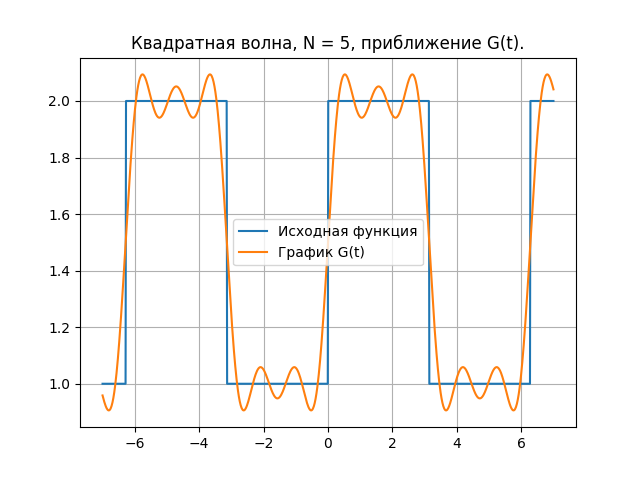
\includegraphics[width=1\linewidth]{gr_wave/g5.png} \\ б)}
\end{minipage}
\caption{Построение графиков частичных сумм, для квадратной волны, $N=5$.}
\end{figure}

\begin{figure}[h]
\begin{minipage}[h]{0.5\linewidth}
\center{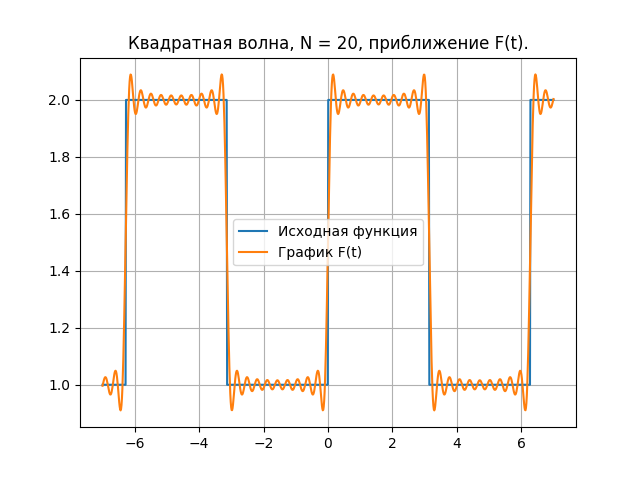
\includegraphics[width=1\linewidth]{gr_wave/f20.png} \\ а)}
\end{minipage}
\hfill
\begin{minipage}[h]{0.5\linewidth}
\center{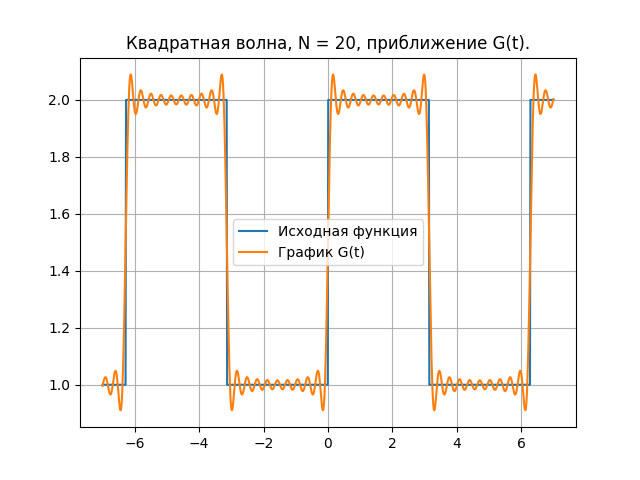
\includegraphics[width=1\linewidth]{gr_wave/g20.png} \\ б)}
\end{minipage}
\caption{Построение графиков частичных сумм, для квадратной волны, $N=20$.}

\begin{minipage}[h]{0.5\linewidth}
\center{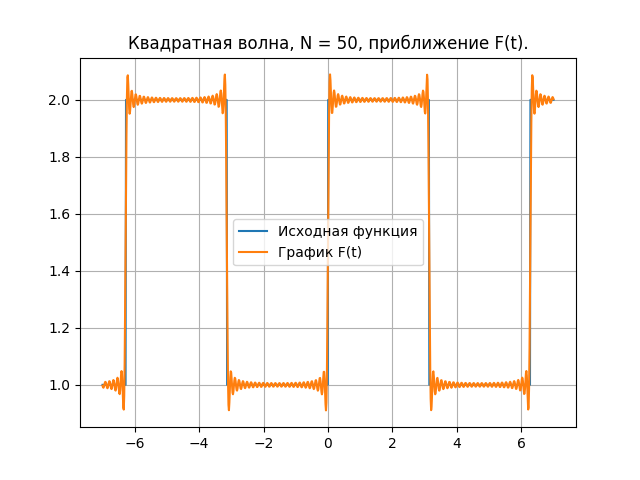
\includegraphics[width=1\linewidth]{gr_wave/f50.png} \\ а)}
\end{minipage}
\hfill
\begin{minipage}[h]{0.5\linewidth}
\center{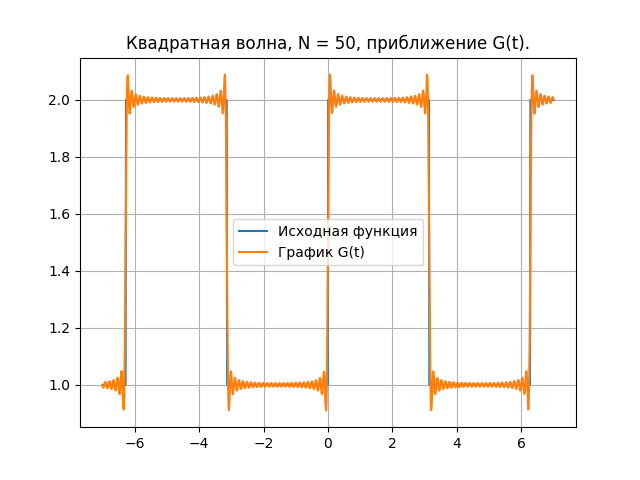
\includegraphics[width=1\linewidth]{gr_wave/g50.png} \\ б)}
\end{minipage}
\caption{Построение графиков частичных сумм, для квадратной волны, $N=50$.}
\end{figure}


При малых значениях $N$ (рис. 2-4) можно заметить, что суммы $F_N(t)$ и $G_N(t)$ практически неотличимы друг от друга.





\newpage
\,
\newpage

На рисунках 2-6 можно заметить, что при увеличении $N$ точность приближения исходного графика функции с помощью частичных сумм Фурье повышается, причем синхронно и неотличимо друг от друга. При $N \geq 5$ суммы Фурье очерчивают очень похожую на исходную функцию.

\subsubsection{Равенство Парсеваля}

Запишем равенство Парсеваля для $F_N$:
\begin{equation}
\| f \|^2 = \pi \left( \frac{a_0^2}{2} + \sum \limits_{n=1}^{\infty} \left( a_n^2 + b_n^2 \right) \right)
\end{equation}

и для $G_N$:

\begin{equation}
\| f \|^2 = 2 \pi \sum \limits_{n = -\infty}^{\infty} |c_n |^2,
\end{equation}
где $\| f \|^2 = \int_a^b (f(t))^2 dt $.
\\
Проведем численную проверку того, что равенство выполнено, для этого напишем новые функции на $Python$. \\
В результате получим выполнение равенства уже при $N=100$, при округлении полученных значений до сотых. В выводе программы получаем:
\begin{equation*}
 \pi \left( \frac{a_0^2}{2} + \sum \limits_{n=1}^{\infty} \left( a_n^2 + b_n^2 \right) \right) = 15.699401582331111
\end{equation*}

\begin{equation*}
2 \pi \sum \limits_{n = -\infty}^{\infty} |c_n |^2 = 15.699401613754796
\end{equation*}

\begin{equation*}
\| f \|^2  = 15.706078312356812
\end{equation*}

Следовательно, равенство Парсеваля для функции квадратной волны выполнено.






\newpage
\subsection{Любая четная периодическая функция.}
\begin{equation}
f(t) = 4 \cos \left( \sin^2 \left( \frac{t}{2}\right) \right)
\end{equation}

\subsubsection{График функции}
\begin{figure}[h]
\center{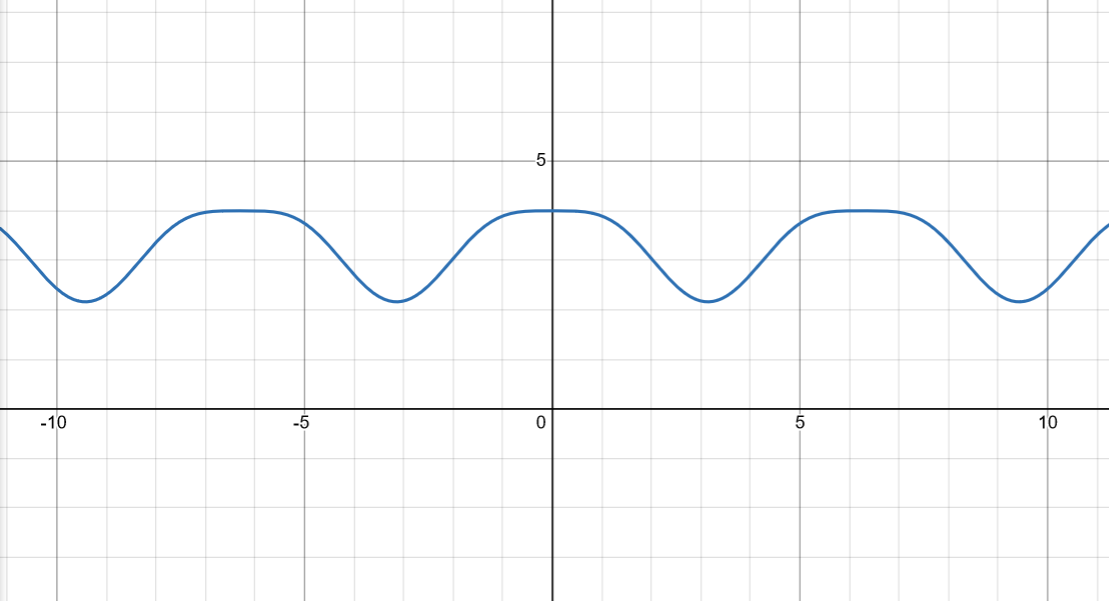
\includegraphics[width=0.9\linewidth]{pic/gr_2.png}}
\caption{График функции $f(t)$.}
\end{figure}

\subsubsection{Частичные суммы Фурье}
Рассмотрим частичные суммы Фурье $F_N$ и $G_N$ вида

\begin{equation}
F_N(t) = \frac{a_0}{2} + \sum  \limits_{n=1}^N \left( a_n \cos \left( \omega_n t \right) + b_n \sin \left( \omega_n t \right)  \right) \, ,
\end{equation}

\begin{equation}
G_N (t) = \sum  \limits_{n=-N}^N c_n e^{i \omega_n t} \, ,
\end{equation}
где $\omega_n = 2 \pi \frac{n}{T}$.\\
\\
Аналогично, $T = 2 \pi$, следовательно, $\omega_n = n$:

\begin{equation}
F_N(t) = \frac{a_0}{2} + \sum  \limits_{n=1}^N \left( a_n \cos \left( n t \right) + b_n \sin \left( n t \right)  \right) \, ,
\end{equation}

\begin{equation}
G_N (t) = \sum  \limits_{n=-N}^N c_n e^{i n t} \, ,
\end{equation}

\subsubsection{Вычисление коэффициентов $a_n$, $b_n$ и $c_n$}
Запишем формулы для вычислия коэффициентов $a_n$, $b_n$ и $c_n$ :

\begin{equation}
a_n = \frac{2}{T} \int \limits_{h}^{h + T} f(t) \cos (nt) dt =  \frac{1}{\pi}\int \limits_{-\pi}^{\pi} 4 \cos \left( \sin^2 \left( \frac{t}{2}\right) \right) \cos (nt) dt 
\end{equation}

\begin{equation}
b_n = \frac{2}{T} \int \limits_{h}^{h + T} f(t) \sin (nt) dt =  \frac{1}{\pi}\int \limits_{-\pi}^{\pi} 4 \cos \left( \sin^2 \left( \frac{t}{2}\right) \right) \sin (nt) dt 
\end{equation}

\begin{equation}
c_n = \frac{1}{T} \int \limits_{h}^{h + T} f(t) e^{-i \omega_n t} dt = \frac{1}{2 \pi} \int \limits_{-\pi}^{\pi} 4 \cos \left( \sin^2 \left( \frac{t}{2}\right) \right) e^{-i n t} dt 
\end{equation}

Вычисление интеграллов в данном случае возможно только численно, так как интегралы, содержащиеся в коэффициентах являются неберущимися. Найдем первые 3 значения:\\
\\
$n = 0:$

\begin{equation}
a_0 = \frac{1}{\pi}\int \limits_{-\pi}^{\pi} 4 \cos \left( \sin^2 \left( \frac{t}{2}\right) \right) dt = 6.58868
\end{equation}

\begin{equation}
b_0 =  \frac{1}{\pi}\int \limits_{-\pi}^{\pi} 4 \cos \left( \sin^2 \left( \frac{t}{2}\right) \right) \sin (0 \cdot t) dt = 0
\end{equation}

\begin{equation}
c_0 = \frac{1}{2 \pi} \int \limits_{-\pi}^{\pi} 4 \cos \left( \sin^2 \left( \frac{t}{2}\right) \right) e^{-i \cdot 0 \cdot t} dt = 3.29434
\end{equation}

$n = 1:$

\begin{equation}
a_1  =  \frac{1}{\pi}\int \limits_{-\pi}^{\pi} 4 \cos \left( \sin^2 \left( \frac{t}{2}\right) \right) \cos (t) dt = 0.929197
\end{equation}

\begin{equation}
b_1 =  \frac{1}{\pi}\int \limits_{-\pi}^{\pi} 4 \cos \left( \sin^2 \left( \frac{t}{2}\right) \right) \sin (t) dt  = 0
\end{equation}

\begin{equation}
c_1 = \frac{1}{2 \pi} \int \limits_{-\pi}^{\pi} 4 \cos \left( \sin^2 \left( \frac{t}{2}\right) \right) e^{-i t} dt = 0.464599
\end{equation}

$n = 2:$

\begin{equation}
a_2 =  \frac{1}{\pi}\int \limits_{-\pi}^{\pi} 4 \cos \left( \sin^2 \left( \frac{t}{2}\right) \right) \cos (2t) dt = -0.21486
\end{equation}

\begin{equation}
b_2 =  \frac{1}{\pi}\int \limits_{-\pi}^{\pi} 4 \cos \left( \sin^2 \left( \frac{t}{2}\right) \right) \sin (2t) dt = 0
\end{equation}

\begin{equation}
c_2 = \frac{1}{2 \pi} \int \limits_{-\pi}^{\pi} 4 \cos \left( \sin^2 \left( \frac{t}{2}\right) \right) e^{-2i t} dt = -0.10743
\end{equation}


\subsubsection{Программа для вычисления коэффициентов Фурье}
Программа аналогична той, которая использовалась для случая квадратной волны, поэтому приведем здесь лишь вычисленные значения для первых трех $n$.

\begin{table}[h]
\caption{Значения коэффициентов, вычисленных с помощью написанной программы для четной периодической функции.}
\label{tabular:timesandtenses}
\begin{center}
\begin{tabular}{|c|c|c|c|c|}
\hline
n & $a_n$ & $b_n$ & $Re(c_n)$ & $Im(c_n)$ \\
\hline
0 & 6.5885 & 0 & 3.2942 & 0\\
\hline
1 & 0.9287 & 0 & 0.4643 & 0\\
\hline
2 & -0.2144 & 0 & -0.1072  & 0\\
\hline
\end{tabular}
\end{center}
\end{table}

Для четной функции так же легко убедиться, что численные значения близки к полученным аналитическим путем (сложные интегралы в этом случае были посчитаны с помощью \textit{Wolfram}).

\subsubsection{Построение графиков частичных сумм $F_N$, $G_N$}

\begin{figure}[h]
\begin{minipage}[h]{0.5\linewidth}
\center{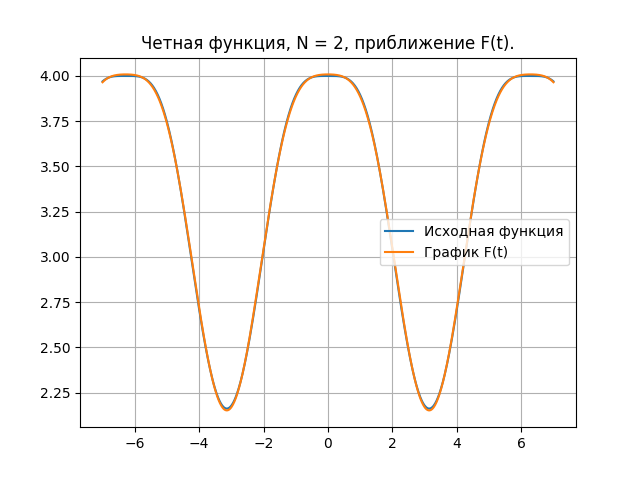
\includegraphics[width=1\linewidth]{gr_even/f2.png} \\ а)}
\end{minipage}
\hfill
\begin{minipage}[h]{0.5\linewidth}
\center{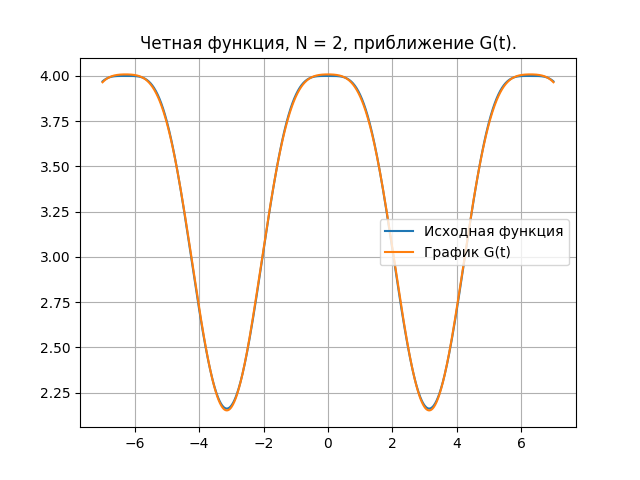
\includegraphics[width=1\linewidth]{gr_even/g2.png} \\ б)}
\end{minipage}
\caption{Построение графиков частичных сумм, для четной функции, $N=2$.}
\vfill

\begin{minipage}[h]{0.5\linewidth}
\center{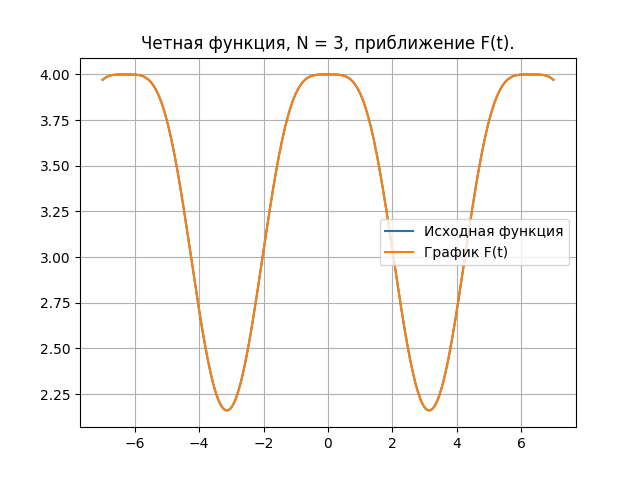
\includegraphics[width=1\linewidth]{gr_even/f3.png} \\ а)}
\end{minipage}
\hfill
\begin{minipage}[h]{0.5\linewidth}
\center{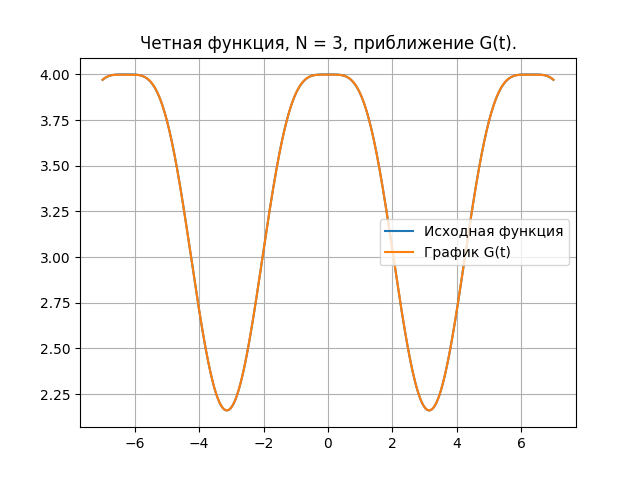
\includegraphics[width=1\linewidth]{gr_even/g3.png} \\ б)}
\end{minipage}
\caption{Построение графиков частичных сумм, для четной функции, $N=3$.}
\end{figure}

\begin{figure}[h]

\begin{minipage}[h]{0.5\linewidth}
\center{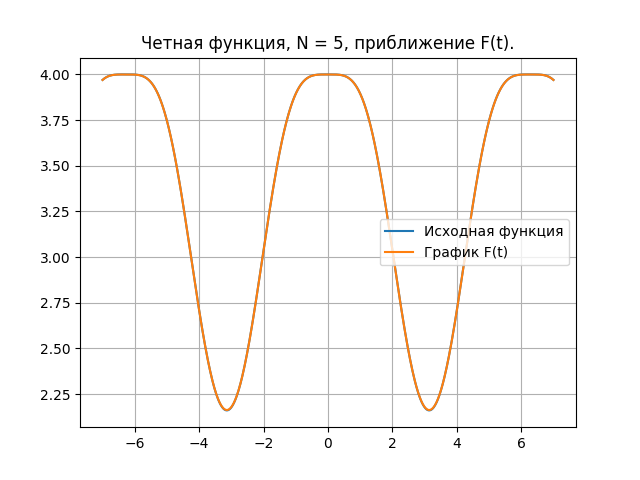
\includegraphics[width=1\linewidth]{gr_even/f5.png} \\ а)}
\end{minipage}
\hfill
\begin{minipage}[h]{0.5\linewidth}
\center{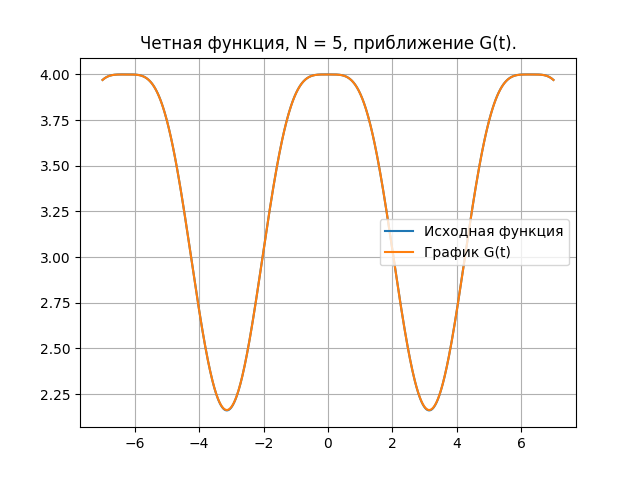
\includegraphics[width=1\linewidth]{gr_even/g5.png} \\ б)}
\end{minipage}
\caption{Построение графиков частичных сумм, для четной функции, $N=5$.}

\vfill
\begin{minipage}[h]{0.5\linewidth}
\center{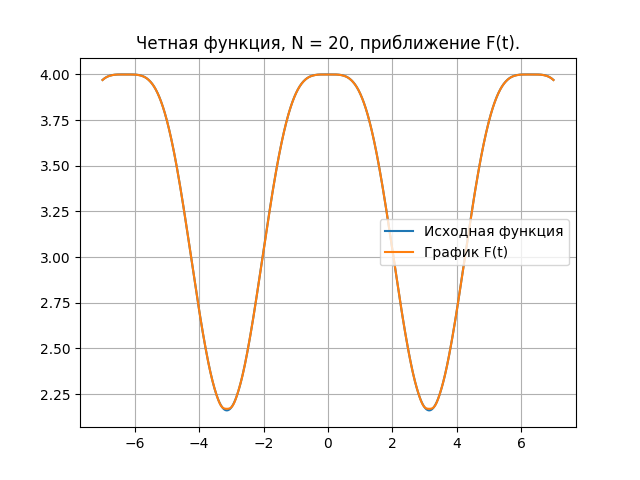
\includegraphics[width=1\linewidth]{gr_even/f20.png} \\ а)}
\end{minipage}
\hfill
\begin{minipage}[h]{0.5\linewidth}
\center{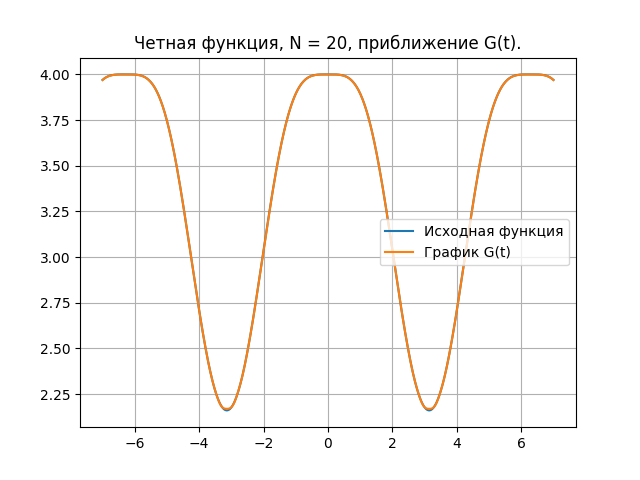
\includegraphics[width=1\linewidth]{gr_even/g20.png} \\ б)}
\end{minipage}
\caption{Построение графиков частичных сумм, для четной функции, $N=20$.}
\end{figure}
\begin{figure}[h]


\begin{minipage}[h]{0.5\linewidth}
\center{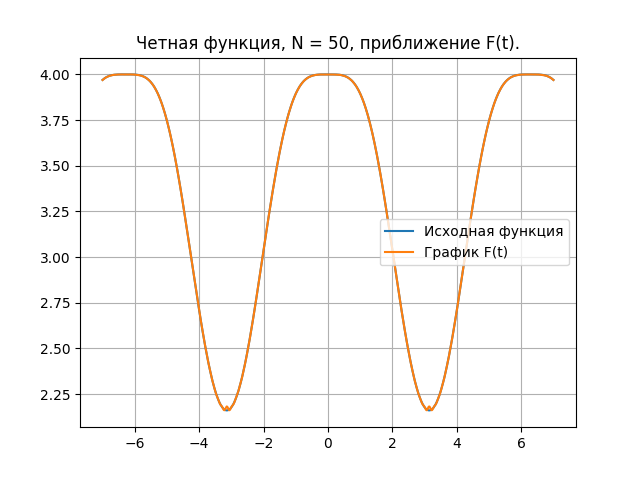
\includegraphics[width=1\linewidth]{gr_even/f50.png} \\ а)}
\end{minipage}
\hfill
\begin{minipage}[h]{0.5\linewidth}
\center{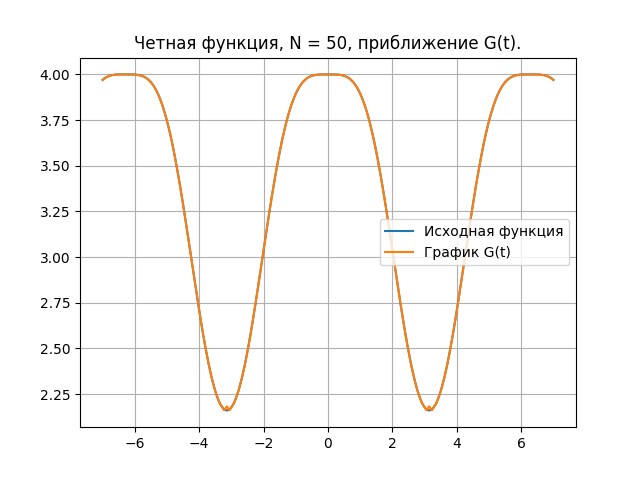
\includegraphics[width=1\linewidth]{gr_even/g50.png} \\ б)}
\end{minipage}
\caption{Построение графиков частичных сумм, для четной функции, $N=50$.}
\end{figure}

Для функции $4 \cos \left( \sin^2 \left( \frac{t}{2}\right) \right)$ суммы $F_N$ и $G_N$ с высокой точностью приближают исходную функцию уже при минимальном $N=2$. 
\newpage
\,
\newpage
\subsubsection{Равенство Парсеваля}

Вновь запишем равенство Парсеваля для $F_N$:
\begin{equation}
\| f \|^2 = \pi \left( \frac{a_0^2}{2} + \sum \limits_{n=1}^{\infty} \left( a_n^2 + b_n^2 \right) \right)
\end{equation}

и для $G_N$:

\begin{equation}
\| f \|^2 = 2 \pi \sum \limits_{n = -\infty}^{\infty} |c_n |^2,
\end{equation}
где $\| f \|^2 = \int_a^b (f(t))^2 dt $.
\\
 В выводе программы при $N=10$ получаем:
\begin{equation*}
 \pi \left( \frac{a_0^2}{2} + \sum \limits_{n=1}^{\infty} \left( a_n^2 + b_n^2 \right) \right) = 71.03881254047784
\end{equation*}

\begin{equation*}
2 \pi \sum \limits_{n = -\infty}^{\infty} |c_n |^2 = 71.03881312743097 
\end{equation*}

\begin{equation*}
\| f \|^2  = 71.04297678948326 
\end{equation*}

Следовательно, равенство Парсеваля для четной функции выполнено. Вновь результаты вычислений оказались равны с точностью до сотых.














\newpage
\subsection{Любая нечетная периодическая функция.}
\begin{equation}
f(t) = \sin^3(t)
\end{equation}

\subsubsection{График функции}
\begin{figure}[h]
\center{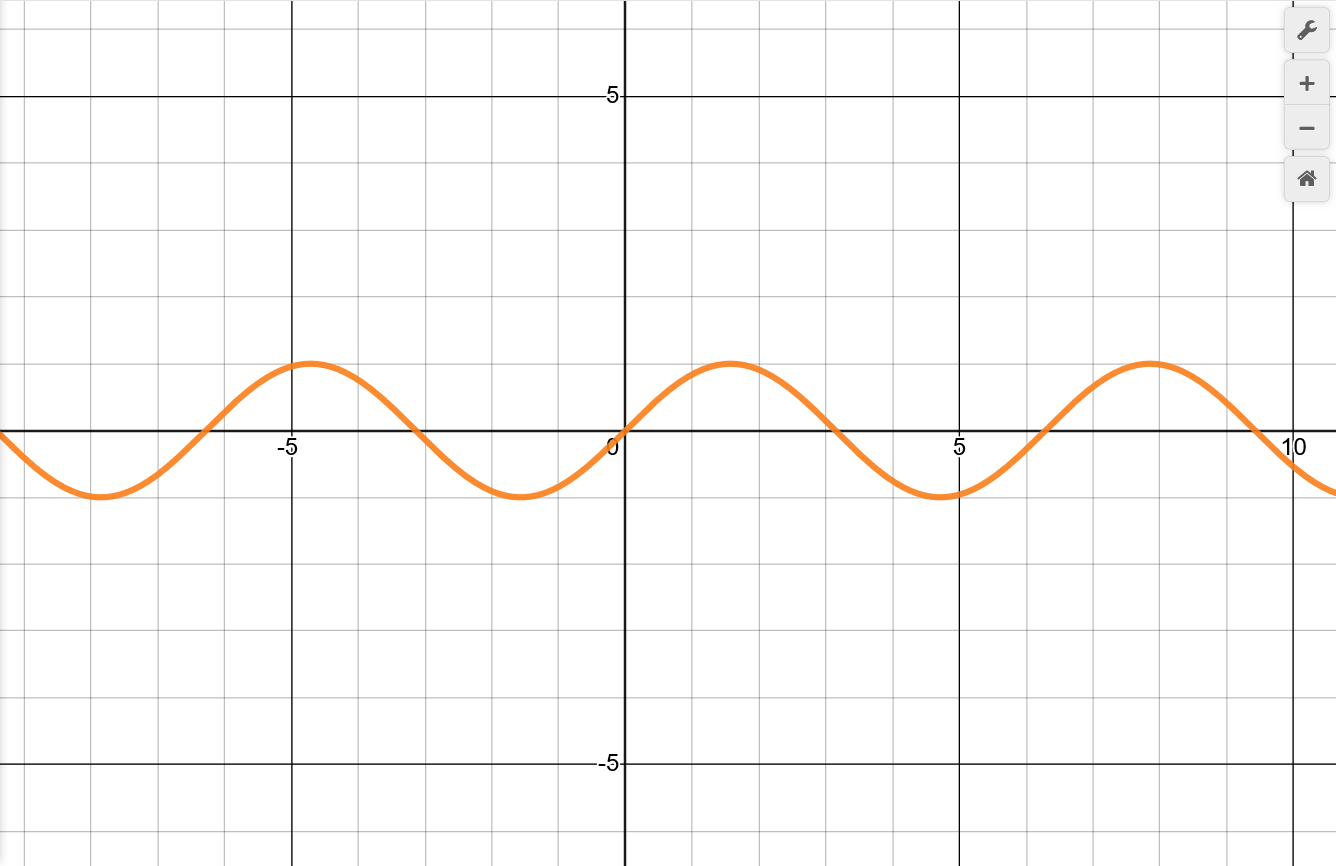
\includegraphics[width=0.9\linewidth]{pic/gr_3.png}}
\caption{График функции $f(t)$.}
\end{figure}

\subsubsection{Частичные суммы Фурье}
Рассмотрим частичные суммы Фурье $F_N$ и $G_N$ вида

\begin{equation}
F_N(t) = \frac{a_0}{2} + \sum  \limits_{n=1}^N \left( a_n \cos \left( \omega_n t \right) + b_n \sin \left( \omega_n t \right)  \right) \, ,
\end{equation}

\begin{equation}
G_N (t) = \sum  \limits_{n=-N}^N c_n e^{i \omega_n t} \, ,
\end{equation}
где $\omega_n = 2 \pi \frac{n}{T}$.\\
\\
Аналогично, $T = 2 \pi$, следовательно, $\omega_n = n$:

\begin{equation}
F_N(t) = \frac{a_0}{2} + \sum  \limits_{n=1}^N \left( a_n \cos \left( n t \right) + b_n \sin \left( n t \right)  \right) \, ,
\end{equation}

\begin{equation}
G_N (t) = \sum  \limits_{n=-N}^N c_n e^{i n t} \, ,
\end{equation}





\subsubsection{Вычисление коэффициентов $a_n$, $b_n$ и $c_n$}

Запишем формулы для вычислия коэффициентов $a_n$, $b_n$ и $c_n$ :

\begin{equation}
a_0 =  \frac{2}{T} \int \limits_{h}^{h + T} f(t) dt =   \frac{1}{\pi} \int \limits_{-\pi}^{\pi} \sin^3(t) dt = 0
\end{equation}


\begin{equation}
a_n = \frac{2}{T} \int \limits_{h}^{h + T} f(t) \cos (nt) dt =  \frac{1}{\pi} \int \limits_{-\pi}^{\pi} \sin^3(t) \cos (nt) dt = 0
\end{equation}

\begin{equation}
b_n = \frac{2}{T} \int \limits_{h}^{h + T} f(t) \sin (nt) dt =  \frac{1}{\pi} \int \limits_{-\pi}^{\pi} \sin^3(t) \sin (nt) dt 
\end{equation}

\begin{equation}
c_n = \frac{1}{T} \int \limits_{h}^{h + T} f(t) e^{-i \omega_n t} dt =  \frac{1}{2 \pi} \int \limits_{-\pi}^{\pi} \sin^3(t) e^{-i n t} dt  
\end{equation}

Найдем численные значения коэффициентов для первых нескольких $n$. \\
\\
$n = 0:$
\begin{equation}
a_0  = 0
\end{equation}

\begin{equation}
b_0  = 0
\end{equation}

\begin{equation}
c_0  = 0
\end{equation}
\\
\\

$n = 1:$
\begin{equation}
a_1 = 0
\end{equation}

\begin{equation}
b_1 = \frac{3}{4}
\end{equation}

\begin{equation}
c_1  = - \frac{3 i  }{8}
\end{equation}
\\
\\

$n = 2:$
\begin{equation}
a_2  = 0
\end{equation}

\begin{equation}
b_2 = 0
\end{equation}

\begin{equation}
c_2  = 0
\end{equation}
\\
\\

$n = 3:$
\begin{equation}
a_3  = 0
\end{equation}

\begin{equation}
b_3 = -\frac{1}{4}
\end{equation}

\begin{equation}
c_3  = \frac{i}{8}
\end{equation}

\newpage
\subsubsection{Программа для вычисления коэффициентов Фурье}

Программа для вычисления коэффициентов Фурье идентична, использовавшейся ранее, поэтому приведем численные результаты для первых четырех значений коэффициентов.

\begin{table}[h]
\caption{Значения коэффициентов, вычисленных с помощью написанной программы для нечетной периодической функции.}
\label{tabular:timesandtenses}
\begin{center}
\begin{tabular}{|c|c|c|c|c|}
\hline
n & $a_n$ & $b_n$ & $Re(c_n)$ & $Im(c_n)$ \\
\hline
0 & 0 & 0 & 0 & 0\\
\hline
1 & 0 & 0.74992 & 0 & -0.37496\\
\hline
2 & 0 & 0 & 0  & 0\\
\hline
3 & 0 & -0.24998 & 0  & 0.12499\\
\hline
\end{tabular}
\end{center}
\end{table}

С помощью программы были посчитаны довольно близкие к аналитическим значения коэффициентов.


\subsubsection{Построение графиков частичных сумм $F_N$, $G_N$}

Ниже предствлены графики частичных сумм для нечетной периодической функции $f(t) = \sin^3(t)$:

\begin{figure}[h]
\begin{minipage}[h]{0.5\linewidth}
\center{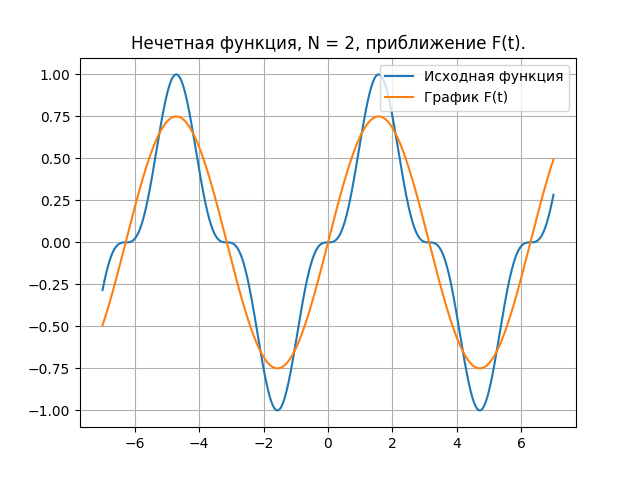
\includegraphics[width=1\linewidth]{gr_odd/f2.png} \\ а)}
\end{minipage}
\hfill
\begin{minipage}[h]{0.5\linewidth}
\center{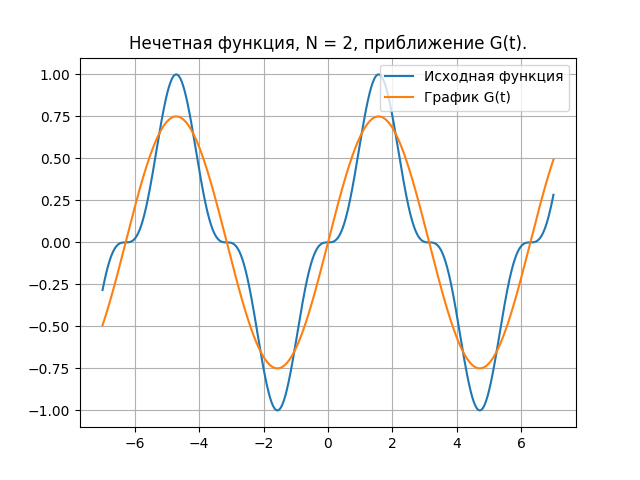
\includegraphics[width=1\linewidth]{gr_odd/g2.png} \\ б)}
\end{minipage}
\caption{Построение графиков частичных сумм, для нечетной функции, $N=2$.}
\end{figure}

\begin{figure}[h]
\begin{minipage}[h]{0.5\linewidth}
\center{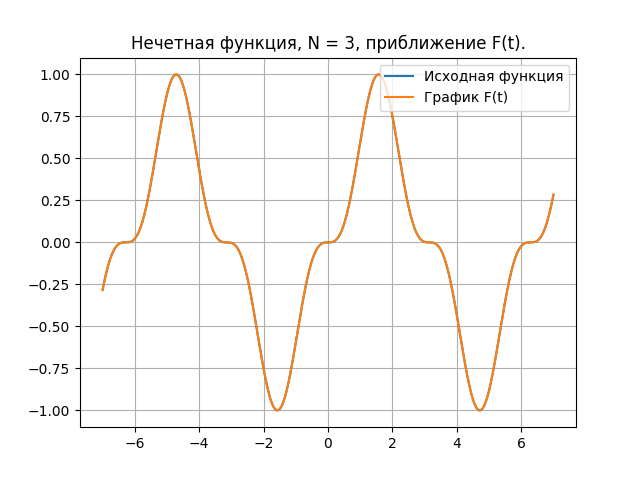
\includegraphics[width=1\linewidth]{gr_odd/f3.png} \\ а)}
\end{minipage}
\hfill
\begin{minipage}[h]{0.5\linewidth}
\center{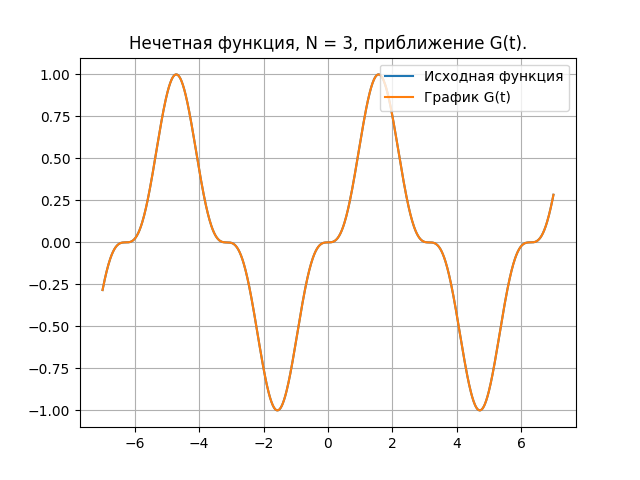
\includegraphics[width=1\linewidth]{gr_odd/g3.png} \\ б)}
\end{minipage}
\caption{Построение графиков частичных сумм, для нечетной функции, $N=3$.}
\vfill

\begin{minipage}[h]{0.5\linewidth}
\center{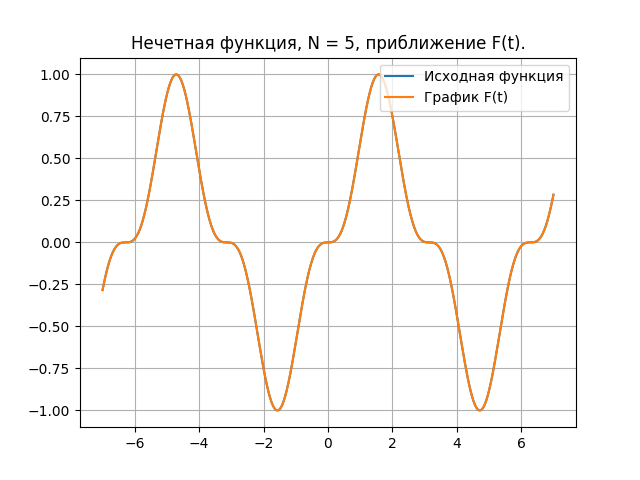
\includegraphics[width=1\linewidth]{gr_odd/f5.png} \\ а)}
\end{minipage}
\hfill
\begin{minipage}[h]{0.5\linewidth}
\center{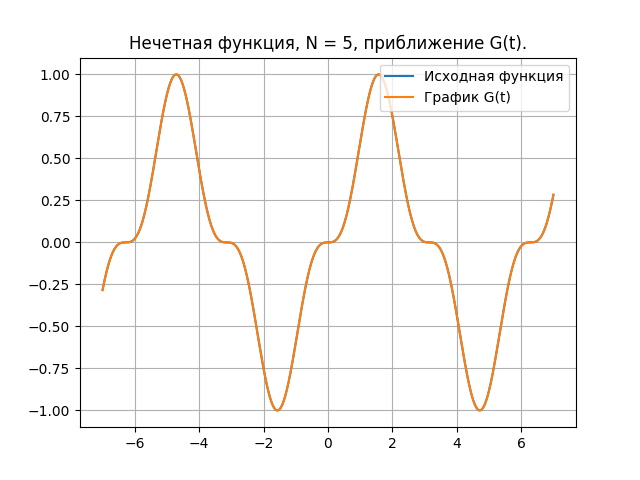
\includegraphics[width=1\linewidth]{gr_odd/g5.png} \\ б)}
\end{minipage}
\caption{Построение графиков частичных сумм, для нечетной функции, $N=5$.}
\end{figure}

\begin{figure}[h]
\begin{minipage}[h]{0.5\linewidth}
\center{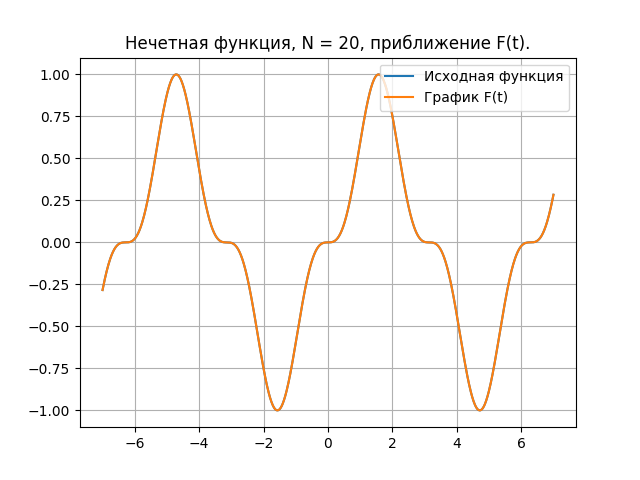
\includegraphics[width=1\linewidth]{gr_odd/f20.png} \\ а)}
\end{minipage}
\hfill
\begin{minipage}[h]{0.5\linewidth}
\center{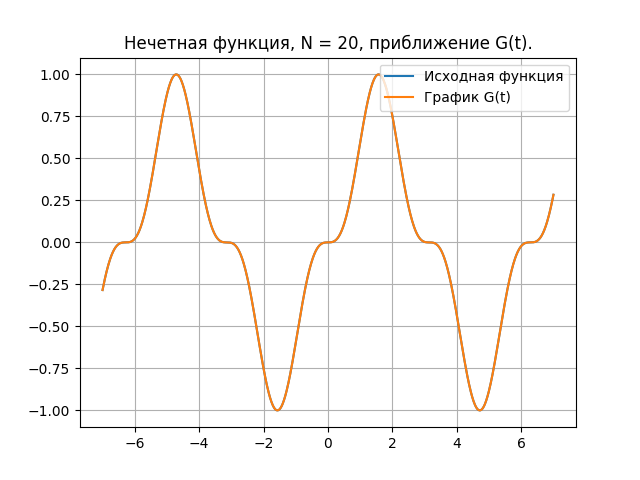
\includegraphics[width=1\linewidth]{gr_odd/g20.png} \\ б)}
\end{minipage}
\caption{Построение графиков частичных сумм, для нечетной функции, $N=20$.}

\begin{minipage}[h]{0.5\linewidth}
\center{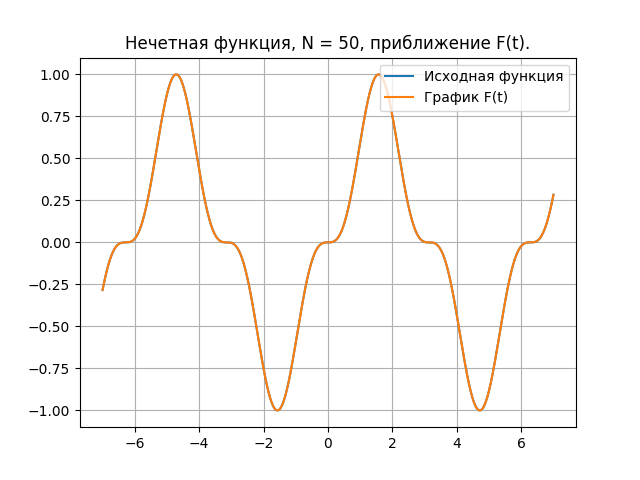
\includegraphics[width=1\linewidth]{gr_odd/f50.png} \\ а)}
\end{minipage}
\hfill
\begin{minipage}[h]{0.5\linewidth}
\center{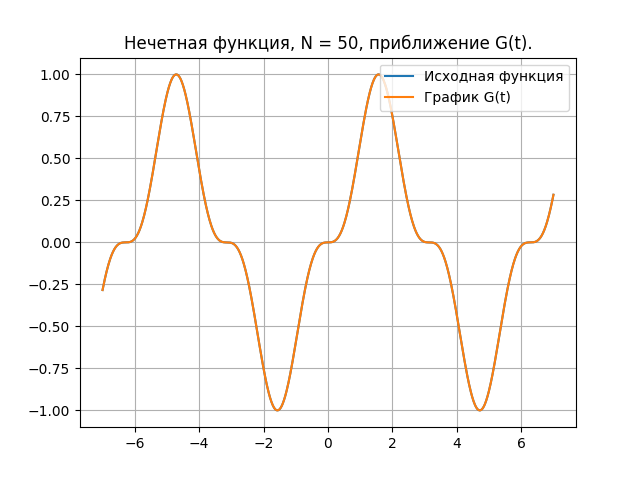
\includegraphics[width=1\linewidth]{gr_odd/g50.png} \\ б)}
\end{minipage}
\caption{Построение графиков частичных сумм, для нечетной функции, $N=50$.}
\end{figure}

Для функции $f(t) = \sin^3(t)$ неотличимыми от исходной функции графики частичных сумм становится с $N=3$, при $N=2$ приближение минимальное (рисунок 14).

\newpage
\,
\newpage
\subsubsection{Равенство Парсеваля}

Вновь запишем равенство Парсеваля для $F_N$:
\begin{equation}
\| f \|^2 = \pi \left( \frac{a_0^2}{2} + \sum \limits_{n=1}^{\infty} \left( a_n^2 + b_n^2 \right) \right)
\end{equation}

и для $G_N$:

\begin{equation}
\| f \|^2 = 2 \pi \sum \limits_{n = -\infty}^{\infty} |c_n |^2,
\end{equation}
где $\| f \|^2 = \int_a^b (f(t))^2 dt $.
\\
\\
 В выводе программы при $N=10$ получаем:
\begin{equation*}
 \pi \left( \frac{a_0^2}{2} + \sum \limits_{n=1}^{\infty} \left( a_n^2 + b_n^2 \right) \right) = 1.9631027290468754 
\end{equation*}

\begin{equation*}
2 \pi \sum \limits_{n = -\infty}^{\infty} |c_n |^2 = 1.963102729046876
\end{equation*}

\begin{equation*}
\| f \|^2  = 1.9632990589527717
\end{equation*}
\\
Следовательно, равенство Парсеваля для нечетной функции выполнено. Результаты вычислений равны с точностью до тысячных.




\newpage
\subsection{Любая периодическая функция, график которой состоит не только из прямых линий, и которая не является ни четной, ни нечетной.}
\begin{equation}
f(t) = \sin(t) - \cos^2(t) 
\end{equation}

\subsubsection{График функции}
\begin{figure}[h]
\center{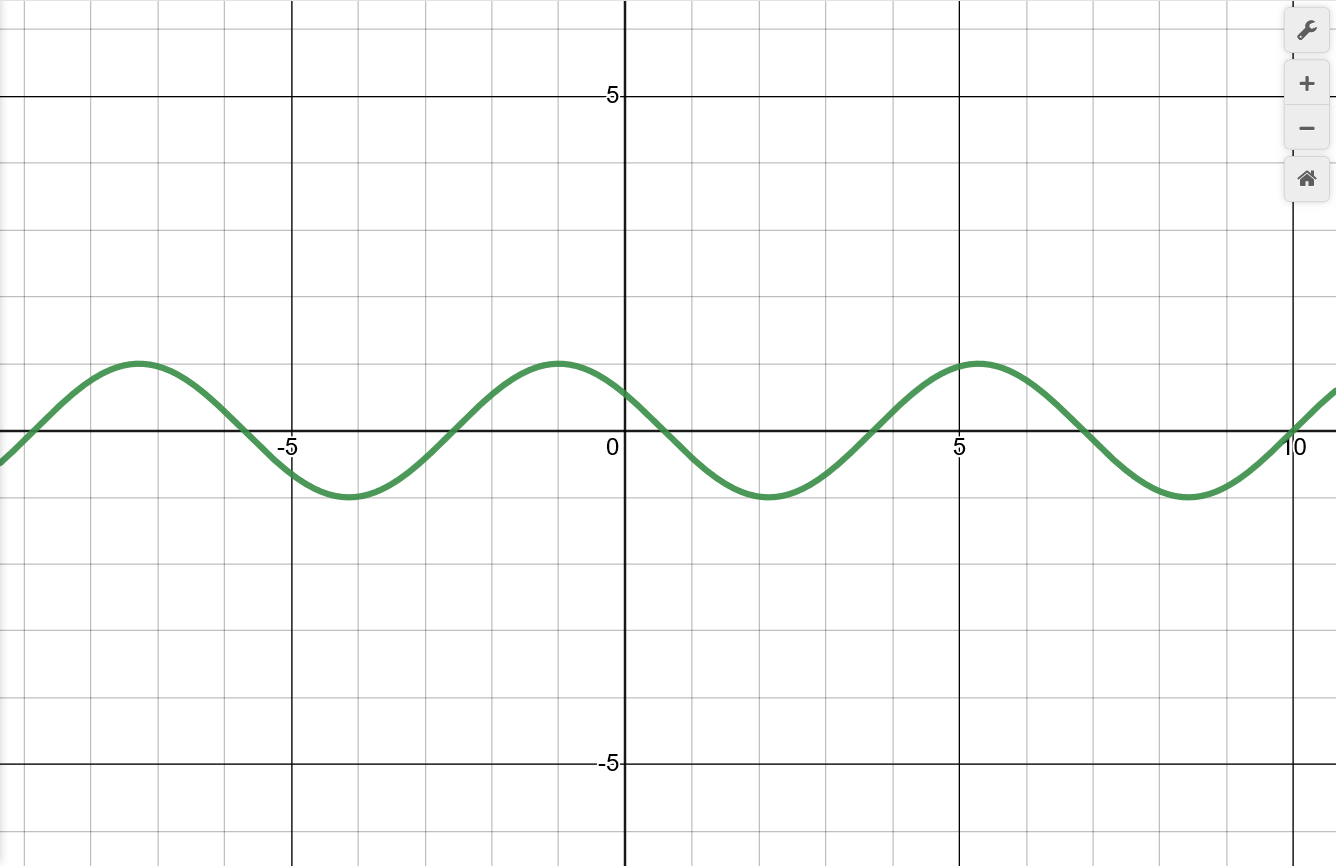
\includegraphics[width=0.9\linewidth]{pic/gr_4.png}}
\caption{График функции $f(t)$.}
\end{figure}

\subsubsection{Частичные суммы Фурье}

Рассмотрим частичные суммы Фурье $F_N$ и $G_N$ вида

\begin{equation}
F_N(t) = \frac{a_0}{2} + \sum  \limits_{n=1}^N \left( a_n \cos \left( \omega_n t \right) + b_n \sin \left( \omega_n t \right)  \right) \, ,
\end{equation}

\begin{equation}
G_N (t) = \sum  \limits_{n=-N}^N c_n e^{i \omega_n t} \, ,
\end{equation}
где $\omega_n = 2 \pi \frac{n}{T}$.\\
\\
Аналогично, $T = 2 \pi$, следовательно, $\omega_n = n$:

\begin{equation}
F_N(t) = \frac{a_0}{2} + \sum  \limits_{n=1}^N \left( a_n \cos \left( n t \right) + b_n \sin \left( n t \right)  \right) \, ,
\end{equation}

\begin{equation}
G_N (t) = \sum  \limits_{n=-N}^N c_n e^{i n t} \, ,
\end{equation}


\subsubsection{Вычисление коэффициентов $a_n$, $b_n$ и $c_n$}

Запишем формулы для вычислия коэффициентов $a_n$, $b_n$ и $c_n$ :

\begin{equation}
a_0 =  \frac{2}{T} \int \limits_{h}^{h + T} f(t) dt =   \frac{1}{\pi} \int \limits_{-\pi}^{\pi} \left( \sin(t) - \cos^2(t) \right) dt = -1
\end{equation}


\begin{equation}
a_n =  \frac{1}{\pi} \int \limits_{-\pi}^{\pi} \left( \sin(t) - \cos^2(t) \right) \cos (nt) dt = -\frac{2(n^2 - 2)\sin(\pi n)}{\pi n (n^2 - 4)}
\end{equation}

\begin{equation}
b_n  =  \frac{1}{\pi} \int \limits_{-\pi}^{\pi} \left( \sin(t) - \cos^2(t) \right) \sin (nt) dt  = \frac{2 \sin (\pi n)}{\pi (1 - n^2)}
\end{equation}

\begin{equation}
c_n =  \frac{1}{2 \pi} \int \limits_{-\pi}^{\pi} \left( \sin(t) - \cos^2(t) \right) e^{-i n t} dt  = \frac{2 }{\pi} \left( \frac{2 - n^2}{n(n^2 - 4)} + \frac{i}{n^2 - 1} \right) \sin (\pi n)
\end{equation}

Найдем численные значения коэффициентов для первых нескольких $n$. \\
\\
$n = 0:$
\begin{equation}
a_0  = -1
\end{equation}

\begin{equation}
b_0  = 0
\end{equation}

\begin{equation}
c_0  = -0.5
\end{equation}
\\
\\

$n = 1:$
\begin{equation}
a_1 = 0
\end{equation}

\begin{equation}
b_1 =  1
\end{equation}

\begin{equation}
c_1  = -0.5 i
\end{equation}
\\
\\

$n = 2:$
\begin{equation}
a_2  = -0.5
\end{equation}

\begin{equation}
b_2 = 0
\end{equation}

\begin{equation}
c_2  = -0.25
\end{equation}
\\

\subsubsection{Программа для вычисления коэффициентов Фурье}

Программа для вычисления коэффициентов Фурье идентична, использовавшейся ранее, поэтому приведем численные результаты для первых трех значений коэффициентов.

\begin{table}[h]
\caption{Значения коэффициентов, вычисленных с помощью написанной программы для ни четной, ни нечетной периодической функции.}
\label{tabular:timesandtenses}
\begin{center}
\begin{tabular}{|c|c|c|c|c|}
\hline
n & $a_n$ & $b_n$ & $Re(c_n)$ & $Im(c_n)$ \\
\hline
0 & -1 & 0 & -0.5 & 0\\
\hline
1 & 0 & 1 & 0 & -0.5\\
\hline
2 & -0.5 & 0 & -0.25  & 0\\
\hline
\end{tabular}
\end{center}
\end{table}

С помощью программы были посчитаны идентичные аналитическим значения коэффициентов.

\subsubsection{Построение графиков частичных сумм $F_N$, $G_N$}

Ниже предствлены графики частичных сумм для ни четной, ни нечетной периодической функции $f(t) = \sin(t) - \cos^2(t)$:

\begin{figure}[h]
\begin{minipage}[h]{0.5\linewidth}
\center{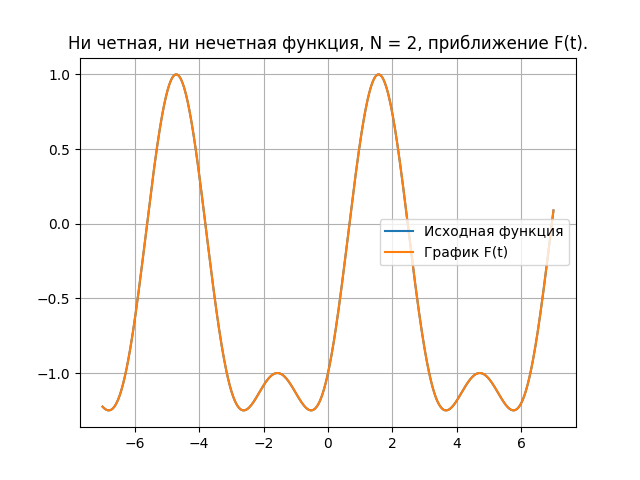
\includegraphics[width=1\linewidth]{gr_neo/f2.png} \\ а)}
\end{minipage}
\hfill
\begin{minipage}[h]{0.5\linewidth}
\center{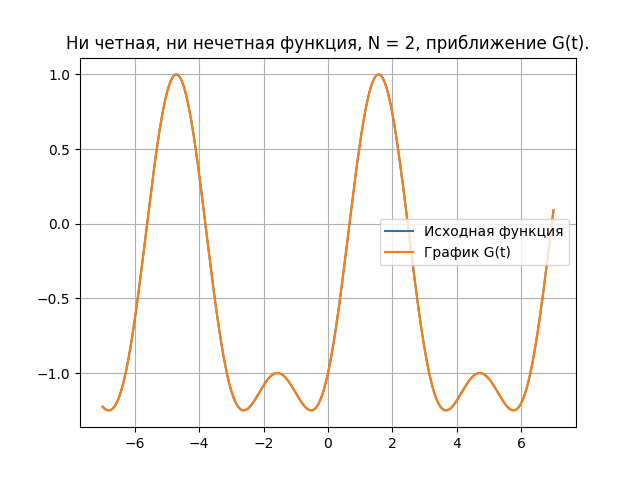
\includegraphics[width=1\linewidth]{gr_neo/g2.png} \\ б)}
\end{minipage}
\caption{Графики частичных сумм для ни чет. ни нечет. функции, $N=2$.}
\vfill
\begin{minipage}[h]{0.5\linewidth}
\center{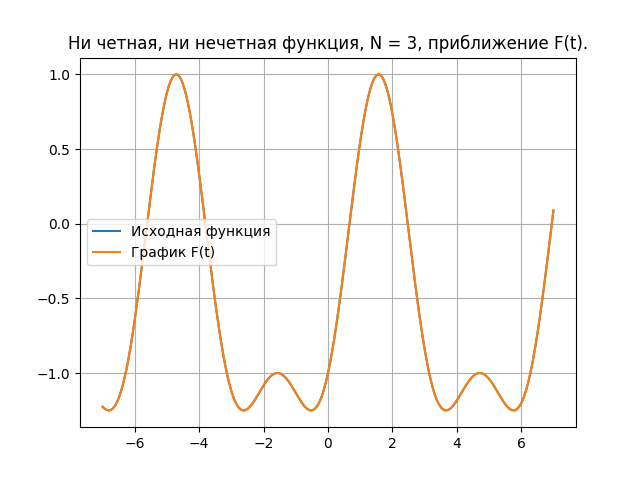
\includegraphics[width=1\linewidth]{gr_neo/f3.png} \\ а)}
\end{minipage}
\hfill
\begin{minipage}[h]{0.5\linewidth}
\center{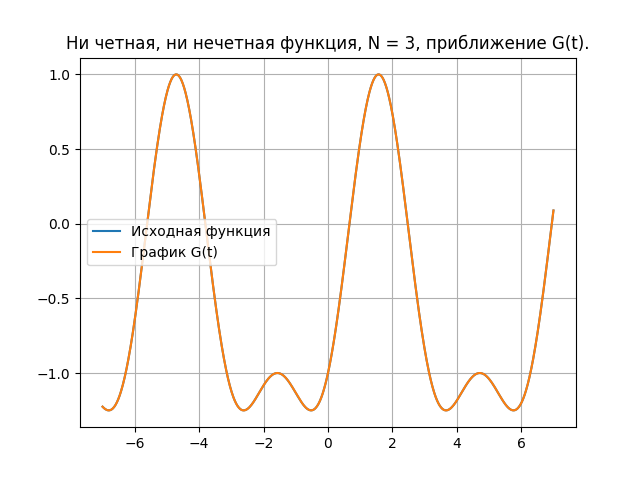
\includegraphics[width=1\linewidth]{gr_neo/g3.png} \\ б)}
\end{minipage}
\caption{Графики частичных сумм для ни чет. ни нечет. функции, $N=3$.}
\end{figure}

\begin{figure}[h]
\begin{minipage}[h]{0.5\linewidth}
\center{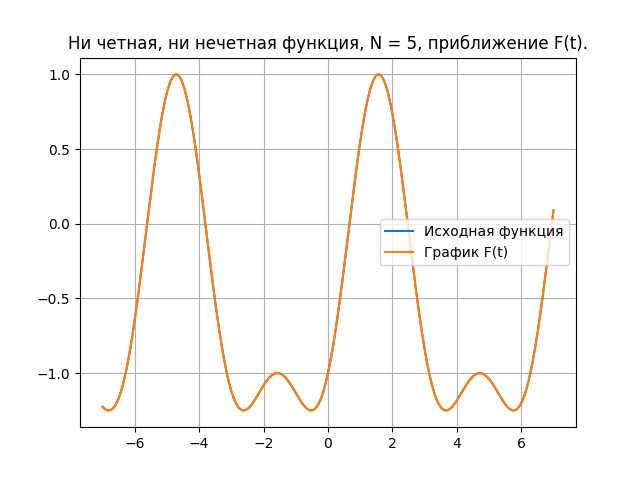
\includegraphics[width=1\linewidth]{gr_neo/f5.png} \\ а)}
\end{minipage}
\hfill
\begin{minipage}[h]{0.5\linewidth}
\center{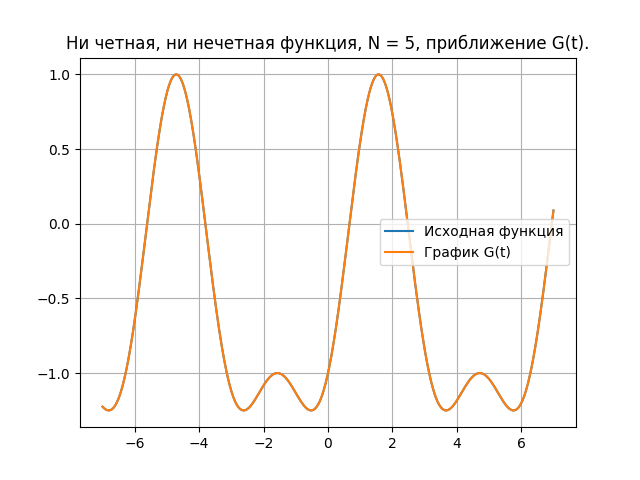
\includegraphics[width=1\linewidth]{gr_neo/g5.png} \\ б)}
\end{minipage}
\caption{Графики частичных сумм для ни чет. ни нечет. функции, $N=5$.}
\vfill
\begin{minipage}[h]{0.5\linewidth}
\center{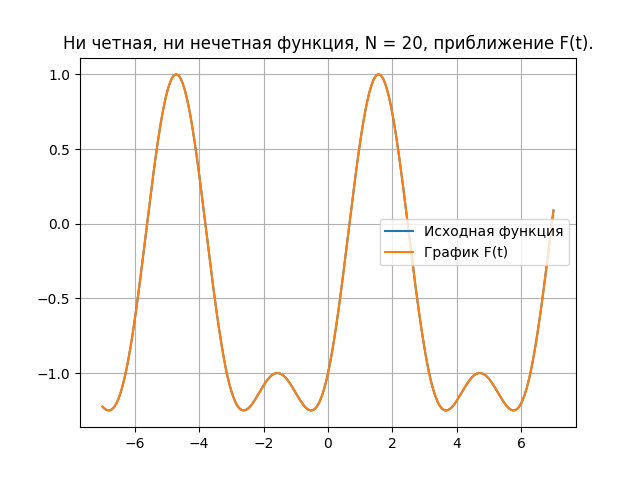
\includegraphics[width=1\linewidth]{gr_neo/f20.png} \\ а)}
\end{minipage}
\hfill
\begin{minipage}[h]{0.5\linewidth}
\center{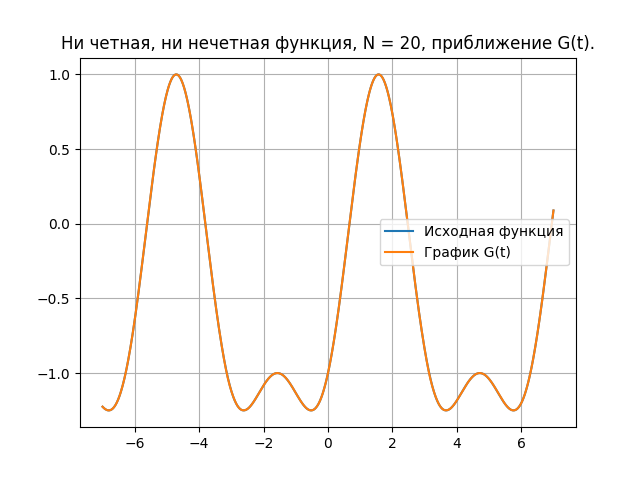
\includegraphics[width=1\linewidth]{gr_neo/g20.png} \\ б)}
\end{minipage}
\caption{Графики частичных сумм для ни чет. ни нечет. функции, $N=20$.}
\end{figure}

\begin{figure}[h]
\begin{minipage}[h]{0.5\linewidth}
\center{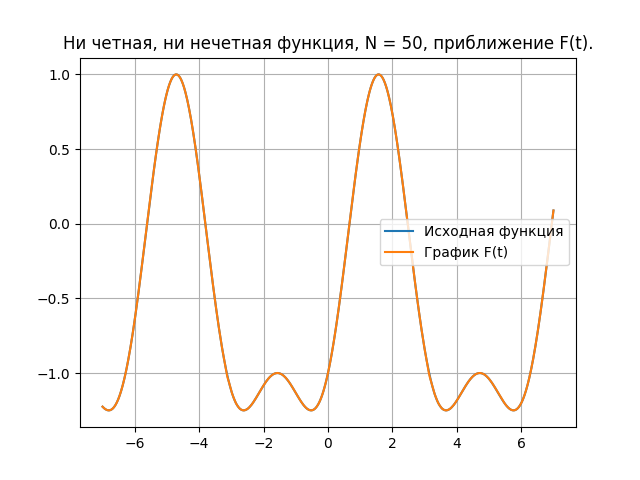
\includegraphics[width=1\linewidth]{gr_neo/f50.png} \\ а)}
\end{minipage}
\hfill
\begin{minipage}[h]{0.5\linewidth}
\center{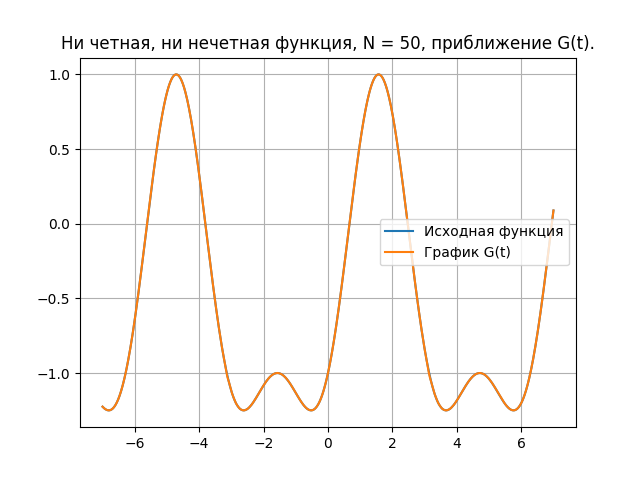
\includegraphics[width=1\linewidth]{gr_neo/g50.png} \\ б)}
\end{minipage}
\caption{Графики частичных сумм для ни чет. ни нечет. функции, $N=50$.}
\end{figure}

Несложно заметить, что уже при значении $N=2$ оба графика частичных сумм практически совпадают с исходной функцией.


\newpage
\,
\newpage
\,

\subsubsection{Равенство Парсеваля}

Вновь запишем равенство Парсеваля для $F_N$:
\begin{equation}
\| f \|^2 = \pi \left( \frac{a_0^2}{2} + \sum \limits_{n=1}^{\infty} \left( a_n^2 + b_n^2 \right) \right)
\end{equation}

и для $G_N$:

\begin{equation}
\| f \|^2 = 2 \pi \sum \limits_{n = -\infty}^{\infty} |c_n |^2,
\end{equation}
где $\| f \|^2 = \int_a^b (f(t))^2 dt $.
\\
\\
 В выводе программы при $N=10$ получаем:
\begin{equation*}
 \pi \left( \frac{a_0^2}{2} + \sum \limits_{n=1}^{\infty} \left( a_n^2 + b_n^2 \right) \right) = 5.497945346534191
\end{equation*}

\begin{equation*}
2 \pi \sum \limits_{n = -\infty}^{\infty} |c_n |^2 = 5.497945472197905
\end{equation*}

\begin{equation*}
\| f \|^2  = 5.497865683598477
\end{equation*}
\\
Следовательно, равенство Парсеваля для ни четной, ни нечетной функции выполнено. Результаты вычислений равны с точностью до четвертого знака после запятой.



\newpage
\section{Задание.}
\subsection{Комплексная функция.}
Зададимся числами $R, \, T > 0$ и рассмотрим комплекснозначную функцию $f : \mathbb{R} \to \mathbb{C}$ с периодом $T$ такую, что
\begin{equation}
Re f(t) =
\begin{cases}
R, & t \in \left[ -\frac{T}{8}, \frac{T}{8} \right)\\
2R - 8Rt / T, &  t \in \left[ \frac{T}{8}, \frac{3T}{8} \right)\\
-R, & t \in \left[ \frac{3T}{8}, \frac{5T}{8} \right)\\
-6R + 8Rt / T, &  t \in \left[ \frac{5T}{8}, \frac{7T}{8} \right)\\
\end{cases}
\,\,\,\,
Im f(t) =
\begin{cases}
8Rt / T, & t \in \left[ -\frac{T}{8}, \frac{T}{8} \right)\\
R, &  t \in \left[ \frac{T}{8}, \frac{3T}{8} \right)\\
4R - 8Rt / T, & t \in \left[ \frac{3T}{8}, \frac{5T}{8} \right)\\
- R, &  t \in \left[ \frac{5T}{8}, \frac{7T}{8} \right)
\end{cases}
\end{equation}


Пусть $R=1$, $T=8$, тогда рассматриваемая функция будет:

\begin{equation}
Re f(t) =
\begin{cases}
1, & t \in \left[ -1, 1 \right)\\
2 - t, &  t \in \left[ 1, 3 \right)\\
-1, & t \in \left[ 3, 5 \right)\\
-6 + t, &  t \in \left[ 5, 7 \right)\\
\end{cases}
\,\,\,\,
Im f(t) =
\begin{cases}
t, & t \in \left[ -1, 1 \right)\\
1, &  t \in \left[ 1, 3 \right)\\
4 - t , & t \in \left[ 3, 5 \right)\\
- 1, &  t \in \left[ 5, 7 \right)
\end{cases}
\end{equation}

\subsubsection{Параметрический график $f(t)$}

\begin{figure}[h]
\center{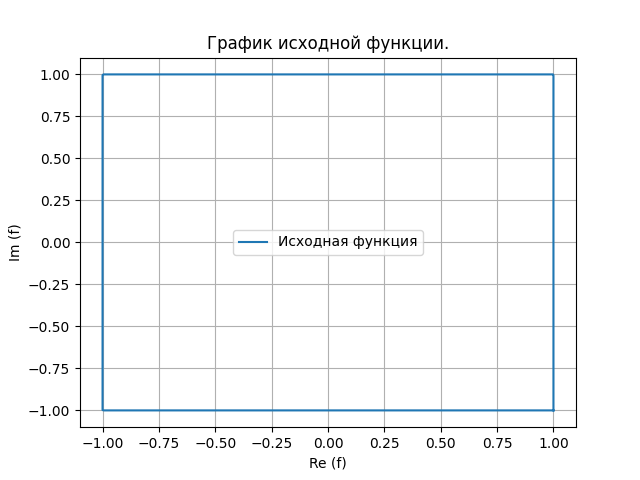
\includegraphics[width=0.68\linewidth]{pic/gr_5.png}}
\caption{График функции $f(t)$.}
\end{figure}

\subsubsection{Частичные суммы Фурье}

\begin{equation}
G_N (t) = \sum  \limits_{n=-N}^N c_n e^{i \omega_n t} \, ,
\end{equation}
где $\omega_n = 2 \pi \frac{n}{T}$.\\
\\
Так как период $T = 8$, то $\omega_n = \frac{\pi n}{4}$ и формула для частичных сумм перепишется в следующем виде:

\begin{equation}
G_N (t) = \sum  \limits_{n=-N}^N c_n e^{i \frac{\pi n}{4} t} \, ,
\end{equation}


\subsubsection{Вычисление коэффициентов $c_n$}
Запишем формулу $c_n$ для произвольного $n$:

\begin{equation}
c_n = \frac{1}{T} \int \limits_{h}^{h + T} f(t) e^{-i \omega_n t} dt 
\end{equation}
И вычислим значение коэффициентов $c_0$, $c_1$, $c_2$ вручную.
\begin{multline*}
c_0 = \frac{1}{8} \int \limits_{-1}^{7} f(t) e^{-i \frac{\pi \cdot 0}{4} t} dt  = \frac{1}{8} \left(\int \limits_{-1}^{1} f(t) dt +
 \int \limits_{1}^{3} f(t) dt + \int \limits_{3}^{5} f(t) dt + \int \limits_{5}^{7} f(t) dt   \right) \fbox{=}
\end{multline*}

\begin{equation}
\int \limits_{-1}^{1} f(t) dt = \int \limits_{-1}^{1} \left( 1 + ti  \right) dt = 2
\end{equation}

\begin{equation}
\int \limits_{1}^{3} f(t) dt = \int \limits_{1}^{3} \left( 2 - t + i  \right) dt = 2i
\end{equation}

\begin{equation}
\int \limits_{3}^{5} f(t) dt = \int \limits_{3}^{5} \left( -1 + (4-t)i  \right) dt = -2
\end{equation}

\begin{equation}
\int \limits_{5}^{7} f(t) dt = \int \limits_{5}^{7} \left( - 6 + t - i \right) dt = -2i
\end{equation}

\begin{equation}
\fbox{=} \frac{1}{8} \left(2 + 2i - 2 - 2i \right) = 0
\end{equation}


\begin{multline*}
c_1 =\frac{1}{8} \left(\int \limits_{-1}^{1} f(t) e^{-i \frac{\pi}{4} t}  dt + \int \limits_{1}^{3} f(t) e^{-i \frac{\pi}{4} t} dt + \int \limits_{3}^{5} f(t) e^{-i \frac{\pi}{4} t}  dt 
+ \int \limits_{5}^{7} f(t) e^{-i \frac{\pi}{4} t}  dt   \right) \fbox{=}
\end{multline*}


\begin{equation}
\int \limits_{-1}^{1} f(t) e^{-i \frac{\pi}{4} t} dt = \int \limits_{-1}^{1} \left( 1 + ti  \right) e^{-i \frac{\pi}{4} t}  dt = \frac{16 \sqrt{2}}{\pi^2} \simeq 2.29264
\end{equation}

\begin{equation}
\int \limits_{1}^{3} f(t)e^{-i \frac{\pi}{4} t} dt = \int \limits_{1}^{3} \left( 2 - t + i  \right) e^{-i \frac{\pi}{4} t} dt = \frac{16 \sqrt{2}}{\pi^2} \simeq 2.29264
\end{equation}

\begin{equation}
\int \limits_{3}^{5} f(t)e^{-i \frac{\pi}{4} t} dt = \int \limits_{3}^{5} \left( -1 + (4-t)i  \right) e^{-i \frac{\pi}{4} t} dt = \frac{16 \sqrt{2}}{\pi^2} \simeq 2.29264
\end{equation}

\begin{equation}
\int \limits_{5}^{7} f(t)e^{-i \frac{\pi}{4} t} dt = \int \limits_{5}^{7} \left( - 6 + t - i \right) e^{-i \frac{\pi}{4} t} dt = \frac{16 \sqrt{2}}{\pi^2} \simeq 2.29264
\end{equation}

\begin{equation}
\fbox{=} \frac{1}{8} \left(\frac{16 \sqrt{2}}{\pi^2} \cdot 4 \right) = \frac{8 \sqrt{2}}{\pi^2} \simeq 1.14632
\end{equation}



\begin{multline*}
c_2 =\frac{1}{8} \left(\int \limits_{-1}^{1} f(t) e^{-i \frac{\pi}{2} t}  dt + \int \limits_{1}^{3} f(t) e^{-i \frac{\pi}{2} t} dt + \int \limits_{3}^{5} f(t) e^{-i \frac{\pi}{2} t}  dt 
+ \int \limits_{5}^{7} f(t) e^{-i \frac{\pi}{2} t}  dt   \right) \fbox{=}
\end{multline*}


\begin{equation}
\int \limits_{-1}^{1} f(t) e^{-i \frac{\pi}{2} t} dt = \int \limits_{-1}^{1} \left( 1 + ti  \right) e^{-i \frac{\pi}{2} t}  dt = \frac{4 (2 + \pi)}{\pi^2} \simeq 2.08381
\end{equation}

\begin{equation}
\int \limits_{1}^{3} f(t)e^{-i \frac{\pi}{2} t} dt = \int \limits_{1}^{3} \left( 2 - t + i  \right) e^{-i \frac{\pi}{2} t} dt = -\frac{4i (2 + \pi)}{\pi^2} \simeq -2.08381i
\end{equation}

\begin{equation}
\int \limits_{3}^{5} f(t)e^{-i \frac{\pi}{2} t} dt = \int \limits_{3}^{5} \left( -1 + (4-t)i  \right) e^{-i \frac{\pi}{2} t} dt = -\frac{4 (2 + \pi)}{\pi^2} \simeq -2.08381
\end{equation}

\begin{equation}
\int \limits_{5}^{7} f(t)e^{-i \frac{\pi}{2} t} dt = \int \limits_{5}^{7} \left( - 6 + t - i \right) e^{-i \frac{\pi}{2} t} dt = \frac{4i (2 + \pi)}{\pi^2} \simeq 2.08381i
\end{equation}

\begin{equation}
\fbox{=} \frac{1}{8} \left(  \frac{4 (2 + \pi)}{\pi^2} -\frac{4i (2 + \pi)}{\pi^2} -\frac{4 (2 + \pi)}{\pi^2} +\frac{4i (2 + \pi)}{\pi^2}  \right) =  0
\end{equation}


\subsubsection{Программа для вычисления коэффициентов Фурье $c_n$}


\begin{center}
\begin{lstlisting}[label=some-code,caption={Функция для коэффициентов $c_n$ комплексной функции}]
# count coefficient c_n for complex fun
def c_complex(f, N):
    res = []
    for n in range(-N, N + 1):
        fourier_exp = lambda t: np.exp(-1j * n * t * np.pi / 4)
        res.append(integral_counter(f, fourier_exp, -1, 7) / 8)
    return res
\end{lstlisting}
\end{center}

\begin{table}[h]
\caption{Значения коэффициентов, вычисленных с помощью написанной программы для коплексной функции.}
\label{tabular:timesandtenses}
\begin{center}
\begin{tabular}{|c|c|c|}
\hline
n &  $Re(c_n)$ & $Im(c_n)$ \\
\hline
0 & 0 & 0\\
\hline
1  & 1.14632 & 0\\
\hline
2  & 0  & 0\\
\hline
\end{tabular}
\end{center}
\end{table}
\newpage
Примечательно, что значения коэффициентов, вычисленных с помощью программы идентичны найденным выше аналитическим способом.

\subsubsection{Построение параметрических графиков $G_N(t)$}
Построим параметрические графики $G_N(t)$ для $N = 1, 2, 3, 10$.

\begin{figure}[h]
\center{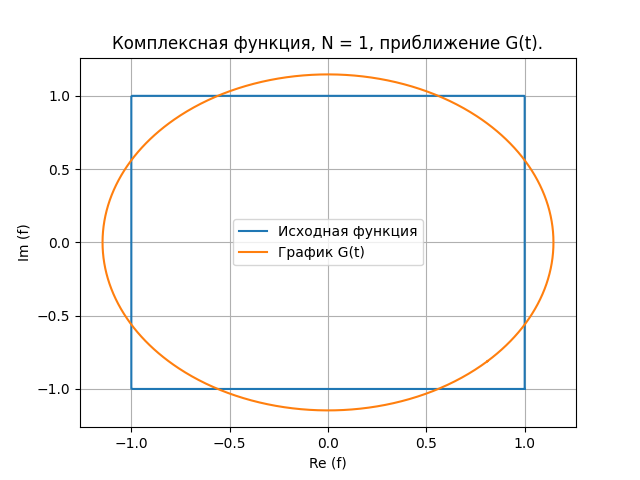
\includegraphics[width=0.85\linewidth]{gr_com/g1.png}}
\caption{График частичной суммы комплексной функции, $N=1$.}
\end{figure}



\begin{figure}[h]
\center{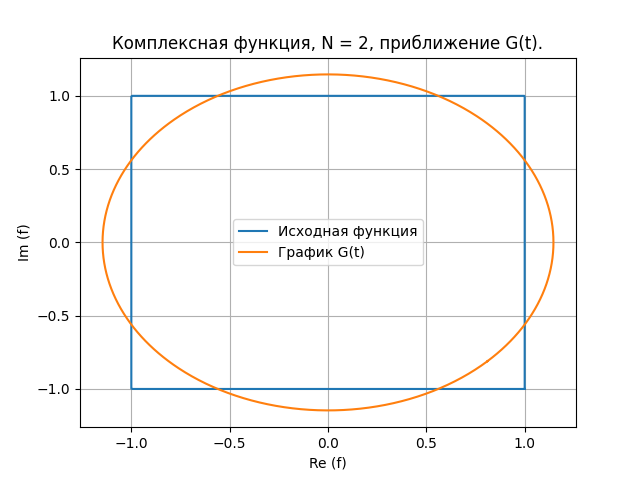
\includegraphics[width=0.85\linewidth]{gr_com/g2.png}}
\caption{График частичной суммы комплексной функции, $N=2$.}
\end{figure}

\begin{figure}[h]
\center{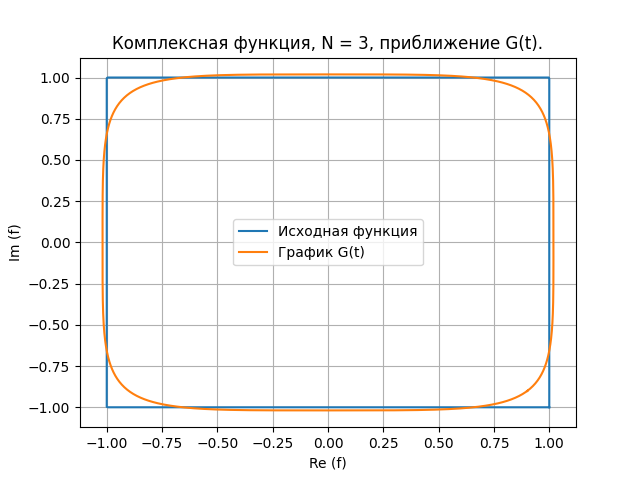
\includegraphics[width=0.85\linewidth]{gr_com/g3.png}}
\caption{График частичной суммы комплексной функции, $N=3$.}
\end{figure}

\begin{figure}[h]
\center{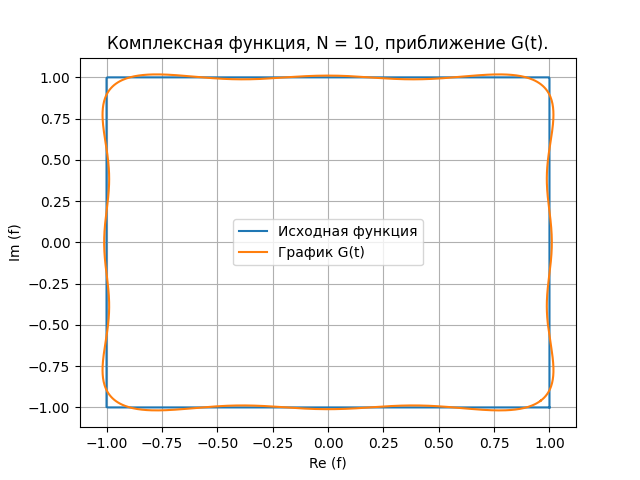
\includegraphics[width=0.85\linewidth]{gr_com/g10.png}}
\caption{График частичной суммы комплексной функции, $N=10$.}
\end{figure}

\newpage
При малых значениях $N = 1, \, 2$ (рисунки 26 - 27) графики частичных сумм слабо приближают график исходной функции и почти не отличаются друг от друга.

\newpage
Начиная с $N=3$ сумма ряда $G_N(t)$ уже точнее описывает график исходной функции, при $N=10$ разница между ними почти незаметна.

\newpage
\,
\newpage
\subsubsection{Построение графиков $Re f(t)$, $Im f(t)$, $Re G_N(t)$ и $Im G_N(t)$}

\begin{figure}[h]
\begin{minipage}[h]{0.5\linewidth}
\center{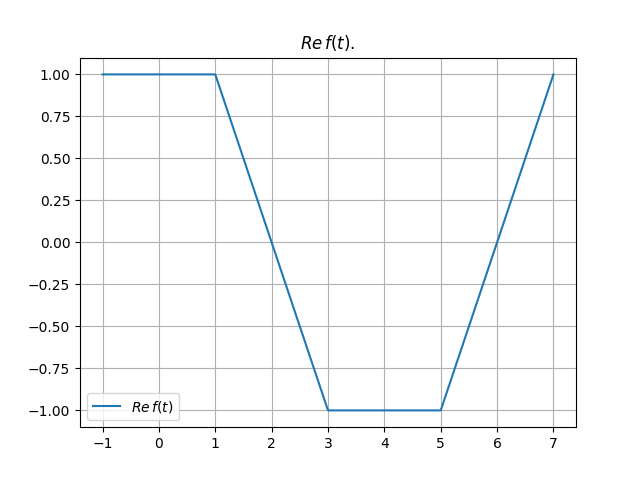
\includegraphics[width=1\linewidth]{rei_com/r_f.png}\\а)}
\end{minipage}
\hfill
\begin{minipage}[h]{0.5\linewidth}
\center{\includegraphics[width=1\linewidth]{rei_com/i_f.png}\\б)}
\end{minipage}
\caption{Графики вещественной и мнимой частей функции $f(t)$.}
\end{figure}

\begin{figure}[h]
\begin{minipage}[h]{0.5\linewidth}
\center{\includegraphics[width=1\linewidth]{rei_com/r_1.png}\\а)}
\end{minipage}
\hfill
\begin{minipage}[h]{0.5\linewidth}
\center{\includegraphics[width=1\linewidth]{rei_com/i_1.png}\\б)}
\end{minipage}
\caption{Графики вещественной и мнимой частей функции $f(t)$ и $G_N$, $N=1$.}
\end{figure}

При $N = 1$, если сравнивать с параметрическим заданием функции, сумма ряда $G_N(t)$ сильнее приближает график исходной функции, как для вещественной, так и для мнимой части.

\begin{figure}[h]
\begin{minipage}[h]{0.5\linewidth}
\center{\includegraphics[width=1\linewidth]{rei_com/r_2.png}\\а)}
\end{minipage}
\hfill
\begin{minipage}[h]{0.5\linewidth}
\center{\includegraphics[width=1\linewidth]{rei_com/i_2.png}\\б)}
\end{minipage}
\caption{Графики вещественной и мнимой частей функции $f(t)$ и $G_N$, $N=2$.}
\end{figure}

\newpage
Для $N=2$ не наблюдается заметных отличий от случая $N=1$ с точки зрения точности приближения исходной функции.

\begin{figure}[h]
\begin{minipage}[h]{0.5\linewidth}
\center{\includegraphics[width=1\linewidth]{rei_com/r_3.png}\\а)}
\end{minipage}
\hfill
\begin{minipage}[h]{0.5\linewidth}
\center{\includegraphics[width=1\linewidth]{rei_com/i_3.png}\\б)}
\end{minipage}
\caption{Графики вещественной и мнимой частей функции $f(t)$ и $G_N$, $N=3$.}
\end{figure}

При $N=3$ точность существенно возрастает и графики практически идентичны, за исключением углов.

\begin{figure}[h]
\begin{minipage}[h]{0.5\linewidth}
\center{\includegraphics[width=1\linewidth]{rei_com/r_10.png}\\а)}
\end{minipage}
\hfill
\begin{minipage}[h]{0.5\linewidth}
\center{\includegraphics[width=1\linewidth]{rei_com/i_10.png}\\б)}
\end{minipage}
\caption{Графики вещественной и мнимой частей функции $f(t)$ и $G_N$, $N=10$.}
\end{figure}

\newpage
В случае $N=10$ график частичной суммы ряда практически неотличим от исходной функции.



\subsubsection{Проверка равенства Парсеваля}

Запишем равенство Парсеваля для $G_N$:

\begin{equation}
\| f \|^2 = 2 \pi \sum \limits_{n = -\infty}^{\infty} |c_n |^2
\end{equation}
\\
\\
 В выводе программы при $N=100$ получаем:
\begin{equation*}
2 \pi \sum \limits_{n = -\infty}^{\infty} |c_n |^2 = 8.376304629985912
\end{equation*}

\begin{equation*}
\| f \|^2  = 8.000040000400004
\end{equation*}
\\
Следовательно, равенство Парсеваля комплексной функции выполнено. Результаты вычислений равны с точностью до целых при $N = 100$.






\section{Дополнительное задание}
\subsection{Произвольный рисунок}

\subsubsection{Задание рисунка на комплексной плоскости}


\subsubsection{Задание "расписания движения" по точкам}


\subsubsection{Коэффициенты соответствующего ряда Фурье}


\subsubsection{Анимация}



%\begin{center}
%\begin{lstlisting}[label=some-code,caption={Исходный код для 1207}]
%\end{lstlisting}
%\end{center}


 
\end{document}













